
% Default to the notebook output style

    


% Inherit from the specified cell style.




    
\documentclass[11pt]{article}

    
    
    \usepackage[T1]{fontenc}
    % Nicer default font (+ math font) than Computer Modern for most use cases
    \usepackage{mathpazo}

    % Basic figure setup, for now with no caption control since it's done
    % automatically by Pandoc (which extracts ![](path) syntax from Markdown).
    \usepackage{graphicx}
    % We will generate all images so they have a width \maxwidth. This means
    % that they will get their normal width if they fit onto the page, but
    % are scaled down if they would overflow the margins.
    \makeatletter
    \def\maxwidth{\ifdim\Gin@nat@width>\linewidth\linewidth
    \else\Gin@nat@width\fi}
    \makeatother
    \let\Oldincludegraphics\includegraphics
    % Set max figure width to be 80% of text width, for now hardcoded.
    \renewcommand{\includegraphics}[1]{\Oldincludegraphics[width=.8\maxwidth]{#1}}
    % Ensure that by default, figures have no caption (until we provide a
    % proper Figure object with a Caption API and a way to capture that
    % in the conversion process - todo).
    \usepackage{caption}
    \DeclareCaptionLabelFormat{nolabel}{}
    \captionsetup{labelformat=nolabel}

    \usepackage{adjustbox} % Used to constrain images to a maximum size 
    \usepackage{xcolor} % Allow colors to be defined
    \usepackage{enumerate} % Needed for markdown enumerations to work
    \usepackage{geometry} % Used to adjust the document margins
    \usepackage{amsmath} % Equations
    \usepackage{amssymb} % Equations
    \usepackage{textcomp} % defines textquotesingle
    % Hack from http://tex.stackexchange.com/a/47451/13684:
    \AtBeginDocument{%
        \def\PYZsq{\textquotesingle}% Upright quotes in Pygmentized code
    }
    \usepackage{upquote} % Upright quotes for verbatim code
    \usepackage{eurosym} % defines \euro
    \usepackage[mathletters]{ucs} % Extended unicode (utf-8) support
    \usepackage[utf8x]{inputenc} % Allow utf-8 characters in the tex document
    \usepackage{fancyvrb} % verbatim replacement that allows latex
    \usepackage{grffile} % extends the file name processing of package graphics 
                         % to support a larger range 
    % The hyperref package gives us a pdf with properly built
    % internal navigation ('pdf bookmarks' for the table of contents,
    % internal cross-reference links, web links for URLs, etc.)
    \usepackage{hyperref}
    \usepackage{longtable} % longtable support required by pandoc >1.10
    \usepackage{booktabs}  % table support for pandoc > 1.12.2
    \usepackage[inline]{enumitem} % IRkernel/repr support (it uses the enumerate* environment)
    \usepackage[normalem]{ulem} % ulem is needed to support strikethroughs (\sout)
                                % normalem makes italics be italics, not underlines
    

    
    
    % Colors for the hyperref package
    \definecolor{urlcolor}{rgb}{0,.145,.698}
    \definecolor{linkcolor}{rgb}{.71,0.21,0.01}
    \definecolor{citecolor}{rgb}{.12,.54,.11}

    % ANSI colors
    \definecolor{ansi-black}{HTML}{3E424D}
    \definecolor{ansi-black-intense}{HTML}{282C36}
    \definecolor{ansi-red}{HTML}{E75C58}
    \definecolor{ansi-red-intense}{HTML}{B22B31}
    \definecolor{ansi-green}{HTML}{00A250}
    \definecolor{ansi-green-intense}{HTML}{007427}
    \definecolor{ansi-yellow}{HTML}{DDB62B}
    \definecolor{ansi-yellow-intense}{HTML}{B27D12}
    \definecolor{ansi-blue}{HTML}{208FFB}
    \definecolor{ansi-blue-intense}{HTML}{0065CA}
    \definecolor{ansi-magenta}{HTML}{D160C4}
    \definecolor{ansi-magenta-intense}{HTML}{A03196}
    \definecolor{ansi-cyan}{HTML}{60C6C8}
    \definecolor{ansi-cyan-intense}{HTML}{258F8F}
    \definecolor{ansi-white}{HTML}{C5C1B4}
    \definecolor{ansi-white-intense}{HTML}{A1A6B2}

    % commands and environments needed by pandoc snippets
    % extracted from the output of `pandoc -s`
    \providecommand{\tightlist}{%
      \setlength{\itemsep}{0pt}\setlength{\parskip}{0pt}}
    \DefineVerbatimEnvironment{Highlighting}{Verbatim}{commandchars=\\\{\}}
    % Add ',fontsize=\small' for more characters per line
    \newenvironment{Shaded}{}{}
    \newcommand{\KeywordTok}[1]{\textcolor[rgb]{0.00,0.44,0.13}{\textbf{{#1}}}}
    \newcommand{\DataTypeTok}[1]{\textcolor[rgb]{0.56,0.13,0.00}{{#1}}}
    \newcommand{\DecValTok}[1]{\textcolor[rgb]{0.25,0.63,0.44}{{#1}}}
    \newcommand{\BaseNTok}[1]{\textcolor[rgb]{0.25,0.63,0.44}{{#1}}}
    \newcommand{\FloatTok}[1]{\textcolor[rgb]{0.25,0.63,0.44}{{#1}}}
    \newcommand{\CharTok}[1]{\textcolor[rgb]{0.25,0.44,0.63}{{#1}}}
    \newcommand{\StringTok}[1]{\textcolor[rgb]{0.25,0.44,0.63}{{#1}}}
    \newcommand{\CommentTok}[1]{\textcolor[rgb]{0.38,0.63,0.69}{\textit{{#1}}}}
    \newcommand{\OtherTok}[1]{\textcolor[rgb]{0.00,0.44,0.13}{{#1}}}
    \newcommand{\AlertTok}[1]{\textcolor[rgb]{1.00,0.00,0.00}{\textbf{{#1}}}}
    \newcommand{\FunctionTok}[1]{\textcolor[rgb]{0.02,0.16,0.49}{{#1}}}
    \newcommand{\RegionMarkerTok}[1]{{#1}}
    \newcommand{\ErrorTok}[1]{\textcolor[rgb]{1.00,0.00,0.00}{\textbf{{#1}}}}
    \newcommand{\NormalTok}[1]{{#1}}
    
    % Additional commands for more recent versions of Pandoc
    \newcommand{\ConstantTok}[1]{\textcolor[rgb]{0.53,0.00,0.00}{{#1}}}
    \newcommand{\SpecialCharTok}[1]{\textcolor[rgb]{0.25,0.44,0.63}{{#1}}}
    \newcommand{\VerbatimStringTok}[1]{\textcolor[rgb]{0.25,0.44,0.63}{{#1}}}
    \newcommand{\SpecialStringTok}[1]{\textcolor[rgb]{0.73,0.40,0.53}{{#1}}}
    \newcommand{\ImportTok}[1]{{#1}}
    \newcommand{\DocumentationTok}[1]{\textcolor[rgb]{0.73,0.13,0.13}{\textit{{#1}}}}
    \newcommand{\AnnotationTok}[1]{\textcolor[rgb]{0.38,0.63,0.69}{\textbf{\textit{{#1}}}}}
    \newcommand{\CommentVarTok}[1]{\textcolor[rgb]{0.38,0.63,0.69}{\textbf{\textit{{#1}}}}}
    \newcommand{\VariableTok}[1]{\textcolor[rgb]{0.10,0.09,0.49}{{#1}}}
    \newcommand{\ControlFlowTok}[1]{\textcolor[rgb]{0.00,0.44,0.13}{\textbf{{#1}}}}
    \newcommand{\OperatorTok}[1]{\textcolor[rgb]{0.40,0.40,0.40}{{#1}}}
    \newcommand{\BuiltInTok}[1]{{#1}}
    \newcommand{\ExtensionTok}[1]{{#1}}
    \newcommand{\PreprocessorTok}[1]{\textcolor[rgb]{0.74,0.48,0.00}{{#1}}}
    \newcommand{\AttributeTok}[1]{\textcolor[rgb]{0.49,0.56,0.16}{{#1}}}
    \newcommand{\InformationTok}[1]{\textcolor[rgb]{0.38,0.63,0.69}{\textbf{\textit{{#1}}}}}
    \newcommand{\WarningTok}[1]{\textcolor[rgb]{0.38,0.63,0.69}{\textbf{\textit{{#1}}}}}
    
    
    % Define a nice break command that doesn't care if a line doesn't already
    % exist.
    \def\br{\hspace*{\fill} \\* }
    % Math Jax compatability definitions
    \def\gt{>}
    \def\lt{<}
    % Document parameters
    \title{Credit Scoring (Part 2)}
    
    
    

    % Pygments definitions
    
\makeatletter
\def\PY@reset{\let\PY@it=\relax \let\PY@bf=\relax%
    \let\PY@ul=\relax \let\PY@tc=\relax%
    \let\PY@bc=\relax \let\PY@ff=\relax}
\def\PY@tok#1{\csname PY@tok@#1\endcsname}
\def\PY@toks#1+{\ifx\relax#1\empty\else%
    \PY@tok{#1}\expandafter\PY@toks\fi}
\def\PY@do#1{\PY@bc{\PY@tc{\PY@ul{%
    \PY@it{\PY@bf{\PY@ff{#1}}}}}}}
\def\PY#1#2{\PY@reset\PY@toks#1+\relax+\PY@do{#2}}

\expandafter\def\csname PY@tok@w\endcsname{\def\PY@tc##1{\textcolor[rgb]{0.73,0.73,0.73}{##1}}}
\expandafter\def\csname PY@tok@c\endcsname{\let\PY@it=\textit\def\PY@tc##1{\textcolor[rgb]{0.25,0.50,0.50}{##1}}}
\expandafter\def\csname PY@tok@cp\endcsname{\def\PY@tc##1{\textcolor[rgb]{0.74,0.48,0.00}{##1}}}
\expandafter\def\csname PY@tok@k\endcsname{\let\PY@bf=\textbf\def\PY@tc##1{\textcolor[rgb]{0.00,0.50,0.00}{##1}}}
\expandafter\def\csname PY@tok@kp\endcsname{\def\PY@tc##1{\textcolor[rgb]{0.00,0.50,0.00}{##1}}}
\expandafter\def\csname PY@tok@kt\endcsname{\def\PY@tc##1{\textcolor[rgb]{0.69,0.00,0.25}{##1}}}
\expandafter\def\csname PY@tok@o\endcsname{\def\PY@tc##1{\textcolor[rgb]{0.40,0.40,0.40}{##1}}}
\expandafter\def\csname PY@tok@ow\endcsname{\let\PY@bf=\textbf\def\PY@tc##1{\textcolor[rgb]{0.67,0.13,1.00}{##1}}}
\expandafter\def\csname PY@tok@nb\endcsname{\def\PY@tc##1{\textcolor[rgb]{0.00,0.50,0.00}{##1}}}
\expandafter\def\csname PY@tok@nf\endcsname{\def\PY@tc##1{\textcolor[rgb]{0.00,0.00,1.00}{##1}}}
\expandafter\def\csname PY@tok@nc\endcsname{\let\PY@bf=\textbf\def\PY@tc##1{\textcolor[rgb]{0.00,0.00,1.00}{##1}}}
\expandafter\def\csname PY@tok@nn\endcsname{\let\PY@bf=\textbf\def\PY@tc##1{\textcolor[rgb]{0.00,0.00,1.00}{##1}}}
\expandafter\def\csname PY@tok@ne\endcsname{\let\PY@bf=\textbf\def\PY@tc##1{\textcolor[rgb]{0.82,0.25,0.23}{##1}}}
\expandafter\def\csname PY@tok@nv\endcsname{\def\PY@tc##1{\textcolor[rgb]{0.10,0.09,0.49}{##1}}}
\expandafter\def\csname PY@tok@no\endcsname{\def\PY@tc##1{\textcolor[rgb]{0.53,0.00,0.00}{##1}}}
\expandafter\def\csname PY@tok@nl\endcsname{\def\PY@tc##1{\textcolor[rgb]{0.63,0.63,0.00}{##1}}}
\expandafter\def\csname PY@tok@ni\endcsname{\let\PY@bf=\textbf\def\PY@tc##1{\textcolor[rgb]{0.60,0.60,0.60}{##1}}}
\expandafter\def\csname PY@tok@na\endcsname{\def\PY@tc##1{\textcolor[rgb]{0.49,0.56,0.16}{##1}}}
\expandafter\def\csname PY@tok@nt\endcsname{\let\PY@bf=\textbf\def\PY@tc##1{\textcolor[rgb]{0.00,0.50,0.00}{##1}}}
\expandafter\def\csname PY@tok@nd\endcsname{\def\PY@tc##1{\textcolor[rgb]{0.67,0.13,1.00}{##1}}}
\expandafter\def\csname PY@tok@s\endcsname{\def\PY@tc##1{\textcolor[rgb]{0.73,0.13,0.13}{##1}}}
\expandafter\def\csname PY@tok@sd\endcsname{\let\PY@it=\textit\def\PY@tc##1{\textcolor[rgb]{0.73,0.13,0.13}{##1}}}
\expandafter\def\csname PY@tok@si\endcsname{\let\PY@bf=\textbf\def\PY@tc##1{\textcolor[rgb]{0.73,0.40,0.53}{##1}}}
\expandafter\def\csname PY@tok@se\endcsname{\let\PY@bf=\textbf\def\PY@tc##1{\textcolor[rgb]{0.73,0.40,0.13}{##1}}}
\expandafter\def\csname PY@tok@sr\endcsname{\def\PY@tc##1{\textcolor[rgb]{0.73,0.40,0.53}{##1}}}
\expandafter\def\csname PY@tok@ss\endcsname{\def\PY@tc##1{\textcolor[rgb]{0.10,0.09,0.49}{##1}}}
\expandafter\def\csname PY@tok@sx\endcsname{\def\PY@tc##1{\textcolor[rgb]{0.00,0.50,0.00}{##1}}}
\expandafter\def\csname PY@tok@m\endcsname{\def\PY@tc##1{\textcolor[rgb]{0.40,0.40,0.40}{##1}}}
\expandafter\def\csname PY@tok@gh\endcsname{\let\PY@bf=\textbf\def\PY@tc##1{\textcolor[rgb]{0.00,0.00,0.50}{##1}}}
\expandafter\def\csname PY@tok@gu\endcsname{\let\PY@bf=\textbf\def\PY@tc##1{\textcolor[rgb]{0.50,0.00,0.50}{##1}}}
\expandafter\def\csname PY@tok@gd\endcsname{\def\PY@tc##1{\textcolor[rgb]{0.63,0.00,0.00}{##1}}}
\expandafter\def\csname PY@tok@gi\endcsname{\def\PY@tc##1{\textcolor[rgb]{0.00,0.63,0.00}{##1}}}
\expandafter\def\csname PY@tok@gr\endcsname{\def\PY@tc##1{\textcolor[rgb]{1.00,0.00,0.00}{##1}}}
\expandafter\def\csname PY@tok@ge\endcsname{\let\PY@it=\textit}
\expandafter\def\csname PY@tok@gs\endcsname{\let\PY@bf=\textbf}
\expandafter\def\csname PY@tok@gp\endcsname{\let\PY@bf=\textbf\def\PY@tc##1{\textcolor[rgb]{0.00,0.00,0.50}{##1}}}
\expandafter\def\csname PY@tok@go\endcsname{\def\PY@tc##1{\textcolor[rgb]{0.53,0.53,0.53}{##1}}}
\expandafter\def\csname PY@tok@gt\endcsname{\def\PY@tc##1{\textcolor[rgb]{0.00,0.27,0.87}{##1}}}
\expandafter\def\csname PY@tok@err\endcsname{\def\PY@bc##1{\setlength{\fboxsep}{0pt}\fcolorbox[rgb]{1.00,0.00,0.00}{1,1,1}{\strut ##1}}}
\expandafter\def\csname PY@tok@kc\endcsname{\let\PY@bf=\textbf\def\PY@tc##1{\textcolor[rgb]{0.00,0.50,0.00}{##1}}}
\expandafter\def\csname PY@tok@kd\endcsname{\let\PY@bf=\textbf\def\PY@tc##1{\textcolor[rgb]{0.00,0.50,0.00}{##1}}}
\expandafter\def\csname PY@tok@kn\endcsname{\let\PY@bf=\textbf\def\PY@tc##1{\textcolor[rgb]{0.00,0.50,0.00}{##1}}}
\expandafter\def\csname PY@tok@kr\endcsname{\let\PY@bf=\textbf\def\PY@tc##1{\textcolor[rgb]{0.00,0.50,0.00}{##1}}}
\expandafter\def\csname PY@tok@bp\endcsname{\def\PY@tc##1{\textcolor[rgb]{0.00,0.50,0.00}{##1}}}
\expandafter\def\csname PY@tok@fm\endcsname{\def\PY@tc##1{\textcolor[rgb]{0.00,0.00,1.00}{##1}}}
\expandafter\def\csname PY@tok@vc\endcsname{\def\PY@tc##1{\textcolor[rgb]{0.10,0.09,0.49}{##1}}}
\expandafter\def\csname PY@tok@vg\endcsname{\def\PY@tc##1{\textcolor[rgb]{0.10,0.09,0.49}{##1}}}
\expandafter\def\csname PY@tok@vi\endcsname{\def\PY@tc##1{\textcolor[rgb]{0.10,0.09,0.49}{##1}}}
\expandafter\def\csname PY@tok@vm\endcsname{\def\PY@tc##1{\textcolor[rgb]{0.10,0.09,0.49}{##1}}}
\expandafter\def\csname PY@tok@sa\endcsname{\def\PY@tc##1{\textcolor[rgb]{0.73,0.13,0.13}{##1}}}
\expandafter\def\csname PY@tok@sb\endcsname{\def\PY@tc##1{\textcolor[rgb]{0.73,0.13,0.13}{##1}}}
\expandafter\def\csname PY@tok@sc\endcsname{\def\PY@tc##1{\textcolor[rgb]{0.73,0.13,0.13}{##1}}}
\expandafter\def\csname PY@tok@dl\endcsname{\def\PY@tc##1{\textcolor[rgb]{0.73,0.13,0.13}{##1}}}
\expandafter\def\csname PY@tok@s2\endcsname{\def\PY@tc##1{\textcolor[rgb]{0.73,0.13,0.13}{##1}}}
\expandafter\def\csname PY@tok@sh\endcsname{\def\PY@tc##1{\textcolor[rgb]{0.73,0.13,0.13}{##1}}}
\expandafter\def\csname PY@tok@s1\endcsname{\def\PY@tc##1{\textcolor[rgb]{0.73,0.13,0.13}{##1}}}
\expandafter\def\csname PY@tok@mb\endcsname{\def\PY@tc##1{\textcolor[rgb]{0.40,0.40,0.40}{##1}}}
\expandafter\def\csname PY@tok@mf\endcsname{\def\PY@tc##1{\textcolor[rgb]{0.40,0.40,0.40}{##1}}}
\expandafter\def\csname PY@tok@mh\endcsname{\def\PY@tc##1{\textcolor[rgb]{0.40,0.40,0.40}{##1}}}
\expandafter\def\csname PY@tok@mi\endcsname{\def\PY@tc##1{\textcolor[rgb]{0.40,0.40,0.40}{##1}}}
\expandafter\def\csname PY@tok@il\endcsname{\def\PY@tc##1{\textcolor[rgb]{0.40,0.40,0.40}{##1}}}
\expandafter\def\csname PY@tok@mo\endcsname{\def\PY@tc##1{\textcolor[rgb]{0.40,0.40,0.40}{##1}}}
\expandafter\def\csname PY@tok@ch\endcsname{\let\PY@it=\textit\def\PY@tc##1{\textcolor[rgb]{0.25,0.50,0.50}{##1}}}
\expandafter\def\csname PY@tok@cm\endcsname{\let\PY@it=\textit\def\PY@tc##1{\textcolor[rgb]{0.25,0.50,0.50}{##1}}}
\expandafter\def\csname PY@tok@cpf\endcsname{\let\PY@it=\textit\def\PY@tc##1{\textcolor[rgb]{0.25,0.50,0.50}{##1}}}
\expandafter\def\csname PY@tok@c1\endcsname{\let\PY@it=\textit\def\PY@tc##1{\textcolor[rgb]{0.25,0.50,0.50}{##1}}}
\expandafter\def\csname PY@tok@cs\endcsname{\let\PY@it=\textit\def\PY@tc##1{\textcolor[rgb]{0.25,0.50,0.50}{##1}}}

\def\PYZbs{\char`\\}
\def\PYZus{\char`\_}
\def\PYZob{\char`\{}
\def\PYZcb{\char`\}}
\def\PYZca{\char`\^}
\def\PYZam{\char`\&}
\def\PYZlt{\char`\<}
\def\PYZgt{\char`\>}
\def\PYZsh{\char`\#}
\def\PYZpc{\char`\%}
\def\PYZdl{\char`\$}
\def\PYZhy{\char`\-}
\def\PYZsq{\char`\'}
\def\PYZdq{\char`\"}
\def\PYZti{\char`\~}
% for compatibility with earlier versions
\def\PYZat{@}
\def\PYZlb{[}
\def\PYZrb{]}
\makeatother


    % Exact colors from NB
    \definecolor{incolor}{rgb}{0.0, 0.0, 0.5}
    \definecolor{outcolor}{rgb}{0.545, 0.0, 0.0}



    
    % Prevent overflowing lines due to hard-to-break entities
    \sloppy 
    % Setup hyperref package
    \hypersetup{
      breaklinks=true,  % so long urls are correctly broken across lines
      colorlinks=true,
      urlcolor=urlcolor,
      linkcolor=linkcolor,
      citecolor=citecolor,
      }
    % Slightly bigger margins than the latex defaults
    
    \geometry{verbose,tmargin=1in,bmargin=1in,lmargin=1in,rmargin=1in}
    
    

    \begin{document}
    
    
    \maketitle
    
    

    
    \section{Model Implementation, and
Optimization}\label{model-implementation-and-optimization}

\subsection{Find out correct Hypothesis space (Model Space), given the
training
set}\label{find-out-correct-hypothesis-space-model-space-given-the-training-set}

\begin{itemize}
\tightlist
\item
  Aim towards minimizing the true error on the test set.
\item
  Avoid Overfitting the data on the training set
\end{itemize}

    \subsubsection{Imports}\label{imports}

We will use the standard data science and machine learning libraries in
this project.

    \begin{Verbatim}[commandchars=\\\{\}]
{\color{incolor}In [{\color{incolor}1}]:} \PY{c+c1}{\PYZsh{} Pandas and numpy for data manipulation}
        \PY{k+kn}{import} \PY{n+nn}{pandas} \PY{k}{as} \PY{n+nn}{pd}
        \PY{k+kn}{import} \PY{n+nn}{numpy} \PY{k}{as} \PY{n+nn}{np}
        
        \PY{c+c1}{\PYZsh{} No warnings about setting value on copy of slice}
        \PY{n}{pd}\PY{o}{.}\PY{n}{options}\PY{o}{.}\PY{n}{mode}\PY{o}{.}\PY{n}{chained\PYZus{}assignment} \PY{o}{=} \PY{k+kc}{None}
        \PY{n}{pd}\PY{o}{.}\PY{n}{set\PYZus{}option}\PY{p}{(}\PY{l+s+s1}{\PYZsq{}}\PY{l+s+s1}{display.max\PYZus{}columns}\PY{l+s+s1}{\PYZsq{}}\PY{p}{,} \PY{l+m+mi}{60}\PY{p}{)}
        
        \PY{c+c1}{\PYZsh{} Matplotlib for visualization}
        \PY{k+kn}{import} \PY{n+nn}{matplotlib}\PY{n+nn}{.}\PY{n+nn}{pyplot} \PY{k}{as} \PY{n+nn}{plt}
        \PY{o}{\PYZpc{}}\PY{k}{matplotlib} inline
        
        \PY{c+c1}{\PYZsh{} Set default font size}
        \PY{n}{plt}\PY{o}{.}\PY{n}{rcParams}\PY{p}{[}\PY{l+s+s1}{\PYZsq{}}\PY{l+s+s1}{font.size}\PY{l+s+s1}{\PYZsq{}}\PY{p}{]} \PY{o}{=} \PY{l+m+mi}{24}
        
        \PY{k+kn}{from} \PY{n+nn}{IPython}\PY{n+nn}{.}\PY{n+nn}{core}\PY{n+nn}{.}\PY{n+nn}{pylabtools} \PY{k}{import} \PY{n}{figsize}
        
        \PY{c+c1}{\PYZsh{} Seaborn for visualization}
        \PY{k+kn}{import} \PY{n+nn}{seaborn} \PY{k}{as} \PY{n+nn}{sns}
        \PY{n}{sns}\PY{o}{.}\PY{n}{set}\PY{p}{(}\PY{n}{font\PYZus{}scale} \PY{o}{=} \PY{l+m+mi}{2}\PY{p}{)}
        
        \PY{c+c1}{\PYZsh{} Imputing missing values and scaling values}
        \PY{k+kn}{from} \PY{n+nn}{sklearn}\PY{n+nn}{.}\PY{n+nn}{preprocessing} \PY{k}{import} \PY{n}{Imputer}\PY{p}{,} \PY{n}{MinMaxScaler}
        
        \PY{c+c1}{\PYZsh{} Machine Learning Models}
        \PY{k+kn}{from} \PY{n+nn}{sklearn}\PY{n+nn}{.}\PY{n+nn}{linear\PYZus{}model} \PY{k}{import} \PY{n}{LinearRegression}
        \PY{k+kn}{from} \PY{n+nn}{sklearn}\PY{n+nn}{.}\PY{n+nn}{ensemble} \PY{k}{import} \PY{n}{RandomForestRegressor}\PY{p}{,} \PY{n}{GradientBoostingRegressor}
        \PY{k+kn}{from} \PY{n+nn}{sklearn}\PY{n+nn}{.}\PY{n+nn}{svm} \PY{k}{import} \PY{n}{SVR}
        \PY{k+kn}{from} \PY{n+nn}{sklearn}\PY{n+nn}{.}\PY{n+nn}{neighbors} \PY{k}{import} \PY{n}{KNeighborsRegressor}
        \PY{k+kn}{from} \PY{n+nn}{xgboost} \PY{k}{import} \PY{n}{XGBRegressor}
        
        \PY{c+c1}{\PYZsh{} Hyperparameter tuning}
        \PY{k+kn}{from} \PY{n+nn}{sklearn}\PY{n+nn}{.}\PY{n+nn}{model\PYZus{}selection} \PY{k}{import} \PY{n}{RandomizedSearchCV}\PY{p}{,} \PY{n}{GridSearchCV}
\end{Verbatim}


    \subsubsection{Read in the data, both Train and
test}\label{read-in-the-data-both-train-and-test}

    \begin{Verbatim}[commandchars=\\\{\}]
{\color{incolor}In [{\color{incolor}2}]:} \PY{c+c1}{\PYZsh{} Read in data into dataframes }
        \PY{n}{train\PYZus{}features} \PY{o}{=} \PY{n}{pd}\PY{o}{.}\PY{n}{read\PYZus{}csv}\PY{p}{(}\PY{l+s+s1}{\PYZsq{}}\PY{l+s+s1}{data/training\PYZus{}features.csv}\PY{l+s+s1}{\PYZsq{}}\PY{p}{)}
        \PY{n}{test\PYZus{}features} \PY{o}{=} \PY{n}{pd}\PY{o}{.}\PY{n}{read\PYZus{}csv}\PY{p}{(}\PY{l+s+s1}{\PYZsq{}}\PY{l+s+s1}{data/testing\PYZus{}features.csv}\PY{l+s+s1}{\PYZsq{}}\PY{p}{)}
        \PY{n}{train\PYZus{}labels} \PY{o}{=} \PY{n}{pd}\PY{o}{.}\PY{n}{read\PYZus{}csv}\PY{p}{(}\PY{l+s+s1}{\PYZsq{}}\PY{l+s+s1}{data/training\PYZus{}labels.csv}\PY{l+s+s1}{\PYZsq{}}\PY{p}{,} \PY{n}{names}\PY{o}{=} \PY{p}{[}\PY{l+s+s1}{\PYZsq{}}\PY{l+s+s1}{score}\PY{l+s+s1}{\PYZsq{}}\PY{p}{]}\PY{p}{)}
        \PY{n}{test\PYZus{}labels} \PY{o}{=} \PY{n}{pd}\PY{o}{.}\PY{n}{read\PYZus{}csv}\PY{p}{(}\PY{l+s+s1}{\PYZsq{}}\PY{l+s+s1}{data/testing\PYZus{}labels.csv}\PY{l+s+s1}{\PYZsq{}} \PY{p}{,} \PY{n}{names}\PY{o}{=} \PY{p}{[}\PY{l+s+s1}{\PYZsq{}}\PY{l+s+s1}{score}\PY{l+s+s1}{\PYZsq{}}\PY{p}{]}\PY{p}{)}
        
        \PY{c+c1}{\PYZsh{} Display sizes of data}
        \PY{n+nb}{print}\PY{p}{(}\PY{l+s+s1}{\PYZsq{}}\PY{l+s+s1}{Training Feature Size: }\PY{l+s+s1}{\PYZsq{}}\PY{p}{,} \PY{n}{train\PYZus{}features}\PY{o}{.}\PY{n}{shape}\PY{p}{)}
        \PY{n+nb}{print}\PY{p}{(}\PY{l+s+s1}{\PYZsq{}}\PY{l+s+s1}{Testing Feature Size:  }\PY{l+s+s1}{\PYZsq{}}\PY{p}{,} \PY{n}{test\PYZus{}features}\PY{o}{.}\PY{n}{shape}\PY{p}{)}
        \PY{n+nb}{print}\PY{p}{(}\PY{l+s+s1}{\PYZsq{}}\PY{l+s+s1}{Training Labels Size:  }\PY{l+s+s1}{\PYZsq{}}\PY{p}{,} \PY{n}{train\PYZus{}labels}\PY{o}{.}\PY{n}{shape}\PY{p}{)}
        \PY{n+nb}{print}\PY{p}{(}\PY{l+s+s1}{\PYZsq{}}\PY{l+s+s1}{Testing Labels Size:   }\PY{l+s+s1}{\PYZsq{}}\PY{p}{,} \PY{n}{test\PYZus{}labels}\PY{o}{.}\PY{n}{shape}\PY{p}{)}
\end{Verbatim}


    \begin{Verbatim}[commandchars=\\\{\}]
Training Feature Size:  (69855, 42)
Testing Feature Size:   (29938, 42)
Training Labels Size:   (69855, 1)
Testing Labels Size:    (29938, 1)

    \end{Verbatim}

    \begin{Verbatim}[commandchars=\\\{\}]
{\color{incolor}In [{\color{incolor}3}]:} \PY{n}{train\PYZus{}labels}\PY{o}{.}\PY{n}{head}\PY{p}{(}\PY{l+m+mi}{12}\PY{p}{)}
\end{Verbatim}


\begin{Verbatim}[commandchars=\\\{\}]
{\color{outcolor}Out[{\color{outcolor}3}]:}          score
        0   740.000000
        1   696.000000
        2   715.000000
        3   742.000000
        4   672.000000
        5   737.000000
        6   716.278671
        7   716.278671
        8   672.000000
        9   735.000000
        10  716.000000
        11  722.000000
\end{Verbatim}
            
    \begin{Verbatim}[commandchars=\\\{\}]
{\color{incolor}In [{\color{incolor}4}]:} \PY{n}{figsize}\PY{p}{(}\PY{l+m+mi}{8}\PY{p}{,} \PY{l+m+mi}{8}\PY{p}{)}
        
        \PY{c+c1}{\PYZsh{} Histogram of the Credit Score}
        \PY{n}{plt}\PY{o}{.}\PY{n}{style}\PY{o}{.}\PY{n}{use}\PY{p}{(}\PY{l+s+s1}{\PYZsq{}}\PY{l+s+s1}{fivethirtyeight}\PY{l+s+s1}{\PYZsq{}}\PY{p}{)}
        \PY{n}{plt}\PY{o}{.}\PY{n}{hist}\PY{p}{(}\PY{n}{train\PYZus{}labels}\PY{p}{[}\PY{l+s+s1}{\PYZsq{}}\PY{l+s+s1}{score}\PY{l+s+s1}{\PYZsq{}}\PY{p}{]}\PY{o}{.}\PY{n}{dropna}\PY{p}{(}\PY{p}{)}\PY{p}{,} \PY{n}{bins} \PY{o}{=} \PY{l+m+mi}{100}\PY{p}{)}\PY{p}{;}
        \PY{n}{plt}\PY{o}{.}\PY{n}{xlabel}\PY{p}{(}\PY{l+s+s1}{\PYZsq{}}\PY{l+s+s1}{Score}\PY{l+s+s1}{\PYZsq{}}\PY{p}{)}\PY{p}{;} \PY{n}{plt}\PY{o}{.}\PY{n}{ylabel}\PY{p}{(}\PY{l+s+s1}{\PYZsq{}}\PY{l+s+s1}{Number}\PY{l+s+s1}{\PYZsq{}}\PY{p}{)}\PY{p}{;} 
        \PY{n}{plt}\PY{o}{.}\PY{n}{title}\PY{p}{(}\PY{l+s+s1}{\PYZsq{}}\PY{l+s+s1}{Credit Score Distribution}\PY{l+s+s1}{\PYZsq{}}\PY{p}{)}\PY{p}{;}
\end{Verbatim}


    \begin{center}
    \adjustimage{max size={0.9\linewidth}{0.9\paperheight}}{output_6_0.png}
    \end{center}
    { \hspace*{\fill} \\}
    
    \subsection{Evaluating and Comparing Machine Learning
Models}\label{evaluating-and-comparing-machine-learning-models}

Build \& train, and evalute several machine learning methods for our
supervised regression task. The objective is to determine which model
holds the most promise for further development (such as hyperparameter
tuning).

We are comparing models using the mean absolute error. A baseline model
that guessed the median value of the score was off by an average of 25
points.

    \begin{itemize}
\item ~
  \subsubsection{Scaling Features}\label{scaling-features}
\end{itemize}

This is necessary because features are in different units, and we want
to normalize the features so the units do not affect the algorithm.
Linear Regression and Random Forest do not require feature scaling, but
other methods, such as support vector machines and k nearest neighbors,
do require it because they take into account the Euclidean distance
between observations. For this reason, it is a best practice to scale
features when we are comparing multiple algorithms.

There are two ways to scale features:

\begin{itemize}
\item
  For each value, subtract the mean of the feature and divide by the
  standard deviation of the feature. This is known as standardization
  and results in each feature having a mean of 0 and a standard
  deviation of 1.
\item
  For each value, subtract the minimum value of the feature and divide
  by the maximum minus the minimum for the feature (the range). This
  assures that all the values for a feature are between 0 and 1 and is
  called scaling to a range or normalization.
\end{itemize}

    \begin{Verbatim}[commandchars=\\\{\}]
{\color{incolor}In [{\color{incolor}5}]:} \PY{c+c1}{\PYZsh{}\PYZsh{} Scale both Training and test set}
        
        
        \PY{c+c1}{\PYZsh{} Create the scaler object with a range of 0\PYZhy{}1}
        \PY{n}{scaler} \PY{o}{=} \PY{n}{MinMaxScaler}\PY{p}{(}\PY{n}{feature\PYZus{}range}\PY{o}{=}\PY{p}{(}\PY{l+m+mi}{0}\PY{p}{,} \PY{l+m+mi}{1}\PY{p}{)}\PY{p}{)}
        
        \PY{c+c1}{\PYZsh{} Fit on the training data}
        \PY{n}{scaler}\PY{o}{.}\PY{n}{fit}\PY{p}{(}\PY{n}{train\PYZus{}features}\PY{p}{)}
        
        \PY{c+c1}{\PYZsh{} Transform both the training and testing data}
        \PY{n}{X} \PY{o}{=} \PY{n}{scaler}\PY{o}{.}\PY{n}{transform}\PY{p}{(}\PY{n}{train\PYZus{}features}\PY{p}{)}
        \PY{n}{X\PYZus{}test} \PY{o}{=} \PY{n}{scaler}\PY{o}{.}\PY{n}{transform}\PY{p}{(}\PY{n}{test\PYZus{}features}\PY{p}{)}
\end{Verbatim}


    \begin{Verbatim}[commandchars=\\\{\}]
{\color{incolor}In [{\color{incolor}6}]:} \PY{c+c1}{\PYZsh{} Convert y to one\PYZhy{}dimensional array (vector)}
        \PY{n}{y} \PY{o}{=} \PY{n}{np}\PY{o}{.}\PY{n}{array}\PY{p}{(}\PY{n}{train\PYZus{}labels}\PY{p}{)}\PY{o}{.}\PY{n}{reshape}\PY{p}{(}\PY{p}{(}\PY{o}{\PYZhy{}}\PY{l+m+mi}{1}\PY{p}{,} \PY{p}{)}\PY{p}{)}
        \PY{n}{y\PYZus{}test} \PY{o}{=} \PY{n}{np}\PY{o}{.}\PY{n}{array}\PY{p}{(}\PY{n}{test\PYZus{}labels}\PY{p}{)}\PY{o}{.}\PY{n}{reshape}\PY{p}{(}\PY{p}{(}\PY{o}{\PYZhy{}}\PY{l+m+mi}{1}\PY{p}{,} \PY{p}{)}\PY{p}{)}
\end{Verbatim}


    \subsection{Models to Evaluate}\label{models-to-evaluate}

We will compare five different machine learning models using the great
Scikit-Learn library:

\begin{enumerate}
\def\labelenumi{\arabic{enumi}.}
\tightlist
\item
  Linear Regression
\item
  Support Vector Machine Regression
\item
  Random Forest Regression
\item
  Gradient Boosting Regression
\item
  K-Nearest Neighbors Regression
\end{enumerate}

    \paragraph{Define Functions to calculate error and run on
model}\label{define-functions-to-calculate-error-and-run-on-model}

    \begin{Verbatim}[commandchars=\\\{\}]
{\color{incolor}In [{\color{incolor}7}]:} \PY{c+c1}{\PYZsh{} Function to calculate mean absolute error}
        \PY{k}{def} \PY{n+nf}{mae}\PY{p}{(}\PY{n}{y\PYZus{}true}\PY{p}{,} \PY{n}{y\PYZus{}pred}\PY{p}{)}\PY{p}{:}
            \PY{k}{return} \PY{n}{np}\PY{o}{.}\PY{n}{mean}\PY{p}{(}\PY{n+nb}{abs}\PY{p}{(}\PY{n}{y\PYZus{}true} \PY{o}{\PYZhy{}} \PY{n}{y\PYZus{}pred}\PY{p}{)}\PY{p}{)}
        
        \PY{c+c1}{\PYZsh{} Takes in a model, trains the model, and evaluates the model on the test set}
        \PY{k}{def} \PY{n+nf}{fit\PYZus{}and\PYZus{}evaluate}\PY{p}{(}\PY{n}{model}\PY{p}{)}\PY{p}{:}
            
            \PY{c+c1}{\PYZsh{} Train the model}
            \PY{n}{model}\PY{o}{.}\PY{n}{fit}\PY{p}{(}\PY{n}{X}\PY{p}{,} \PY{n}{y}\PY{p}{)}
            
            \PY{c+c1}{\PYZsh{} Make predictions and evalute}
            \PY{n}{model\PYZus{}pred} \PY{o}{=} \PY{n}{model}\PY{o}{.}\PY{n}{predict}\PY{p}{(}\PY{n}{X\PYZus{}test}\PY{p}{)}
            \PY{n}{model\PYZus{}mae} \PY{o}{=} \PY{n}{mae}\PY{p}{(}\PY{n}{y\PYZus{}test}\PY{p}{,} \PY{n}{model\PYZus{}pred}\PY{p}{)}
            
            \PY{c+c1}{\PYZsh{} Return the performance metric}
            \PY{k}{return} \PY{n}{model\PYZus{}mae}
\end{Verbatim}


    \subsection{Figuring out a Base model to Optimise
on}\label{figuring-out-a-base-model-to-optimise-on}

    \begin{Verbatim}[commandchars=\\\{\}]
{\color{incolor}In [{\color{incolor}8}]:} \PY{n}{lr} \PY{o}{=} \PY{n}{LinearRegression}\PY{p}{(}\PY{p}{)}
        \PY{n}{lr\PYZus{}mae} \PY{o}{=} \PY{n}{fit\PYZus{}and\PYZus{}evaluate}\PY{p}{(}\PY{n}{lr}\PY{p}{)}
        
        \PY{n+nb}{print}\PY{p}{(}\PY{l+s+s1}{\PYZsq{}}\PY{l+s+s1}{Linear Regression Performance on the test set: MAE = }\PY{l+s+si}{\PYZpc{}0.4f}\PY{l+s+s1}{\PYZsq{}} \PY{o}{\PYZpc{}} \PY{n}{lr\PYZus{}mae}\PY{p}{)}
\end{Verbatim}


    \begin{Verbatim}[commandchars=\\\{\}]
Linear Regression Performance on the test set: MAE = 16.8592

    \end{Verbatim}

    \begin{Verbatim}[commandchars=\\\{\}]
{\color{incolor}In [{\color{incolor}9}]:} \PY{n}{random\PYZus{}forest} \PY{o}{=} \PY{n}{RandomForestRegressor}\PY{p}{(}\PY{n}{random\PYZus{}state}\PY{o}{=}\PY{l+m+mi}{60}\PY{p}{)}
        \PY{n}{random\PYZus{}forest\PYZus{}mae} \PY{o}{=} \PY{n}{fit\PYZus{}and\PYZus{}evaluate}\PY{p}{(}\PY{n}{random\PYZus{}forest}\PY{p}{)}
        
        \PY{n+nb}{print}\PY{p}{(}\PY{l+s+s1}{\PYZsq{}}\PY{l+s+s1}{Random Forest Regression Performance on the test set: MAE = }\PY{l+s+si}{\PYZpc{}0.4f}\PY{l+s+s1}{\PYZsq{}} \PY{o}{\PYZpc{}} \PY{n}{random\PYZus{}forest\PYZus{}mae}\PY{p}{)}
\end{Verbatim}


    \begin{Verbatim}[commandchars=\\\{\}]
Random Forest Regression Performance on the test set: MAE = 12.8542

    \end{Verbatim}

    \begin{Verbatim}[commandchars=\\\{\}]
{\color{incolor}In [{\color{incolor}10}]:} \PY{n}{gradient\PYZus{}boosted} \PY{o}{=} \PY{n}{GradientBoostingRegressor}\PY{p}{(}\PY{n}{random\PYZus{}state}\PY{o}{=}\PY{l+m+mi}{60}\PY{p}{)}
         \PY{n}{gradient\PYZus{}boosted\PYZus{}mae} \PY{o}{=} \PY{n}{fit\PYZus{}and\PYZus{}evaluate}\PY{p}{(}\PY{n}{gradient\PYZus{}boosted}\PY{p}{)}
         
         \PY{n+nb}{print}\PY{p}{(}\PY{l+s+s1}{\PYZsq{}}\PY{l+s+s1}{Gradient Boosted Regression Performance on the test set: MAE = }\PY{l+s+si}{\PYZpc{}0.4f}\PY{l+s+s1}{\PYZsq{}} \PY{o}{\PYZpc{}} \PY{n}{gradient\PYZus{}boosted\PYZus{}mae}\PY{p}{)}
\end{Verbatim}


    \begin{Verbatim}[commandchars=\\\{\}]
Gradient Boosted Regression Performance on the test set: MAE = 15.2863

    \end{Verbatim}

    \begin{Verbatim}[commandchars=\\\{\}]
{\color{incolor}In [{\color{incolor}11}]:} \PY{n}{knn} \PY{o}{=} \PY{n}{KNeighborsRegressor}\PY{p}{(}\PY{n}{n\PYZus{}neighbors}\PY{o}{=}\PY{l+m+mi}{10}\PY{p}{)}
         \PY{n}{knn\PYZus{}mae} \PY{o}{=} \PY{n}{fit\PYZus{}and\PYZus{}evaluate}\PY{p}{(}\PY{n}{knn}\PY{p}{)}
         
         \PY{n+nb}{print}\PY{p}{(}\PY{l+s+s1}{\PYZsq{}}\PY{l+s+s1}{K\PYZhy{}Nearest Neighbors Regression Performance on the test set: MAE = }\PY{l+s+si}{\PYZpc{}0.4f}\PY{l+s+s1}{\PYZsq{}} \PY{o}{\PYZpc{}} \PY{n}{knn\PYZus{}mae}\PY{p}{)}
\end{Verbatim}


    \begin{Verbatim}[commandchars=\\\{\}]
K-Nearest Neighbors Regression Performance on the test set: MAE = 17.1680

    \end{Verbatim}

    \begin{Verbatim}[commandchars=\\\{\}]
{\color{incolor}In [{\color{incolor}12}]:} \PY{n}{xgb} \PY{o}{=} \PY{n}{XGBRegressor}\PY{p}{(}\PY{p}{)}
         \PY{n}{xgb\PYZus{}mae} \PY{o}{=} \PY{n}{fit\PYZus{}and\PYZus{}evaluate}\PY{p}{(}\PY{n}{xgb}\PY{p}{)}
         
         \PY{n+nb}{print}\PY{p}{(}\PY{l+s+s1}{\PYZsq{}}\PY{l+s+s1}{XGB Regression Performance on the test set: MAE = }\PY{l+s+si}{\PYZpc{}0.4f}\PY{l+s+s1}{\PYZsq{}} \PY{o}{\PYZpc{}} \PY{n}{xgb\PYZus{}mae}\PY{p}{)}
\end{Verbatim}


    \begin{Verbatim}[commandchars=\\\{\}]
XGB Regression Performance on the test set: MAE = 15.3022

    \end{Verbatim}

    \begin{Verbatim}[commandchars=\\\{\}]
{\color{incolor}In [{\color{incolor}13}]:} \PY{n}{plt}\PY{o}{.}\PY{n}{style}\PY{o}{.}\PY{n}{use}\PY{p}{(}\PY{l+s+s1}{\PYZsq{}}\PY{l+s+s1}{fivethirtyeight}\PY{l+s+s1}{\PYZsq{}}\PY{p}{)}
         \PY{n}{figsize}\PY{p}{(}\PY{l+m+mi}{8}\PY{p}{,} \PY{l+m+mi}{6}\PY{p}{)}
         
         \PY{c+c1}{\PYZsh{} Dataframe to hold the results}
         \PY{n}{model\PYZus{}comparison} \PY{o}{=} \PY{n}{pd}\PY{o}{.}\PY{n}{DataFrame}\PY{p}{(}\PY{p}{\PYZob{}}\PY{l+s+s1}{\PYZsq{}}\PY{l+s+s1}{model}\PY{l+s+s1}{\PYZsq{}}\PY{p}{:} \PY{p}{[}\PY{l+s+s1}{\PYZsq{}}\PY{l+s+s1}{Linear Regression}\PY{l+s+s1}{\PYZsq{}}\PY{p}{,}
                                                    \PY{l+s+s1}{\PYZsq{}}\PY{l+s+s1}{Random Forest}\PY{l+s+s1}{\PYZsq{}}\PY{p}{,} \PY{l+s+s1}{\PYZsq{}}\PY{l+s+s1}{XGBRegressor}\PY{l+s+s1}{\PYZsq{}}\PY{p}{,} \PY{l+s+s1}{\PYZsq{}}\PY{l+s+s1}{Gradient Boosted}\PY{l+s+s1}{\PYZsq{}}\PY{p}{,}
                                                     \PY{l+s+s1}{\PYZsq{}}\PY{l+s+s1}{K\PYZhy{}Nearest Neighbors}\PY{l+s+s1}{\PYZsq{}}\PY{p}{]}\PY{p}{,}
                                          \PY{l+s+s1}{\PYZsq{}}\PY{l+s+s1}{mae}\PY{l+s+s1}{\PYZsq{}}\PY{p}{:} \PY{p}{[}\PY{n}{lr\PYZus{}mae}\PY{p}{,} \PY{n}{random\PYZus{}forest\PYZus{}mae}\PY{p}{,} \PY{n}{xgb\PYZus{}mae}\PY{p}{,}
                                                  \PY{n}{gradient\PYZus{}boosted\PYZus{}mae}\PY{p}{,} \PY{n}{knn\PYZus{}mae}\PY{p}{]}\PY{p}{\PYZcb{}}\PY{p}{)}
         
         \PY{c+c1}{\PYZsh{} Horizontal bar chart of test mae}
         \PY{n}{model\PYZus{}comparison}\PY{o}{.}\PY{n}{sort\PYZus{}values}\PY{p}{(}\PY{l+s+s1}{\PYZsq{}}\PY{l+s+s1}{mae}\PY{l+s+s1}{\PYZsq{}}\PY{p}{,} \PY{n}{ascending} \PY{o}{=} \PY{k+kc}{False}\PY{p}{)}\PY{o}{.}\PY{n}{plot}\PY{p}{(}\PY{n}{x} \PY{o}{=} \PY{l+s+s1}{\PYZsq{}}\PY{l+s+s1}{model}\PY{l+s+s1}{\PYZsq{}}\PY{p}{,} \PY{n}{y} \PY{o}{=} \PY{l+s+s1}{\PYZsq{}}\PY{l+s+s1}{mae}\PY{l+s+s1}{\PYZsq{}}\PY{p}{,} \PY{n}{kind} \PY{o}{=} \PY{l+s+s1}{\PYZsq{}}\PY{l+s+s1}{barh}\PY{l+s+s1}{\PYZsq{}}\PY{p}{,}
                                                                    \PY{n}{color} \PY{o}{=} \PY{l+s+s1}{\PYZsq{}}\PY{l+s+s1}{purple}\PY{l+s+s1}{\PYZsq{}}\PY{p}{,} \PY{n}{edgecolor} \PY{o}{=} \PY{l+s+s1}{\PYZsq{}}\PY{l+s+s1}{black}\PY{l+s+s1}{\PYZsq{}}\PY{p}{)}
         
         \PY{c+c1}{\PYZsh{} Plot formatting}
         \PY{n}{plt}\PY{o}{.}\PY{n}{ylabel}\PY{p}{(}\PY{l+s+s1}{\PYZsq{}}\PY{l+s+s1}{\PYZsq{}}\PY{p}{)}\PY{p}{;} \PY{n}{plt}\PY{o}{.}\PY{n}{yticks}\PY{p}{(}\PY{n}{size} \PY{o}{=} \PY{l+m+mi}{14}\PY{p}{)}\PY{p}{;} \PY{n}{plt}\PY{o}{.}\PY{n}{xlabel}\PY{p}{(}\PY{l+s+s1}{\PYZsq{}}\PY{l+s+s1}{Mean Absolute Error}\PY{l+s+s1}{\PYZsq{}}\PY{p}{)}\PY{p}{;} \PY{n}{plt}\PY{o}{.}\PY{n}{xticks}\PY{p}{(}\PY{n}{size} \PY{o}{=} \PY{l+m+mi}{14}\PY{p}{)}
         \PY{n}{plt}\PY{o}{.}\PY{n}{title}\PY{p}{(}\PY{l+s+s1}{\PYZsq{}}\PY{l+s+s1}{Model Comparison on Test MAE}\PY{l+s+s1}{\PYZsq{}}\PY{p}{,} \PY{n}{size} \PY{o}{=} \PY{l+m+mi}{20}\PY{p}{)}\PY{p}{;}
\end{Verbatim}


    \begin{center}
    \adjustimage{max size={0.9\linewidth}{0.9\paperheight}}{output_20_0.png}
    \end{center}
    { \hspace*{\fill} \\}
    
    Although this is not a fair comparison because all the default
parameters are used in making the models, but from the errors it can be
inferred that the problem is Learnable, because all the models did
significantly better than the baseline error of : 17.626

    \subsection{Model Optimization¶}\label{model-optimization}

In machine learning, optimizing a model means finding the best set of
hyperparameters for a particular problem.

Hyperparameters First off, we need to understand what model
hyperparameters are in contrast to model parameters :

\begin{itemize}
\tightlist
\item
  Model hyperparameters are best thought of as settings for a machine
  learning algorithm that are tuned by the data scientist before
  training. Examples would be the number of trees in the random forest,
  or the number of neighbors used in K Nearest Neighbors Regression.
\item
  Model parameters are what the model learns during training, such as
  the weights in the linear regression.
\end{itemize}

    \subsubsection{Hyperparameter Tuning with Random Search and Cross
Validation}\label{hyperparameter-tuning-with-random-search-and-cross-validation}

We can choose the best hyperparameters for a model through random search
and cross validation.

\begin{itemize}
\item
  Random search refers to the method in which we choose hyperparameters
  to evaluate: we define a range of options, and then randomly select
  combinations to try. This is in contrast to grid search which
  evaluates every single combination we specify. Generally, random
  search is better when we have limited knowledge of the best model
  hyperparameters and we can use random search to narrow down the
  options and then use grid search with a more limited range of options.
\item
  Cross validation is the method used to assess the performance of the
  hyperparameters. Rather than splitting the training set up into
  separate training and validation sets which reduces the amount of
  training data we can use, we use K-Fold Cross Validation. This means
  dividing the training data into K folds, and then going through an
  iterative process where we first train on K-1 of the folds and then
  evaluate performance on the kth fold. We repeat this process K times
  so eventually we will have tested on every example in the training
  data with the key that each iteration we are testing on data that we
  did not train on. At the end of K-fold cross validation, we take the
  average error on each of the K iterations as the final performance
  measure and then train the model on all the training data at once. The
  performance we record is then used to compare different combinations
  of hyperparameters.
\end{itemize}

    A picture of k-fold cross validation using k = 5 is shown below:

    \begin{figure}
\centering
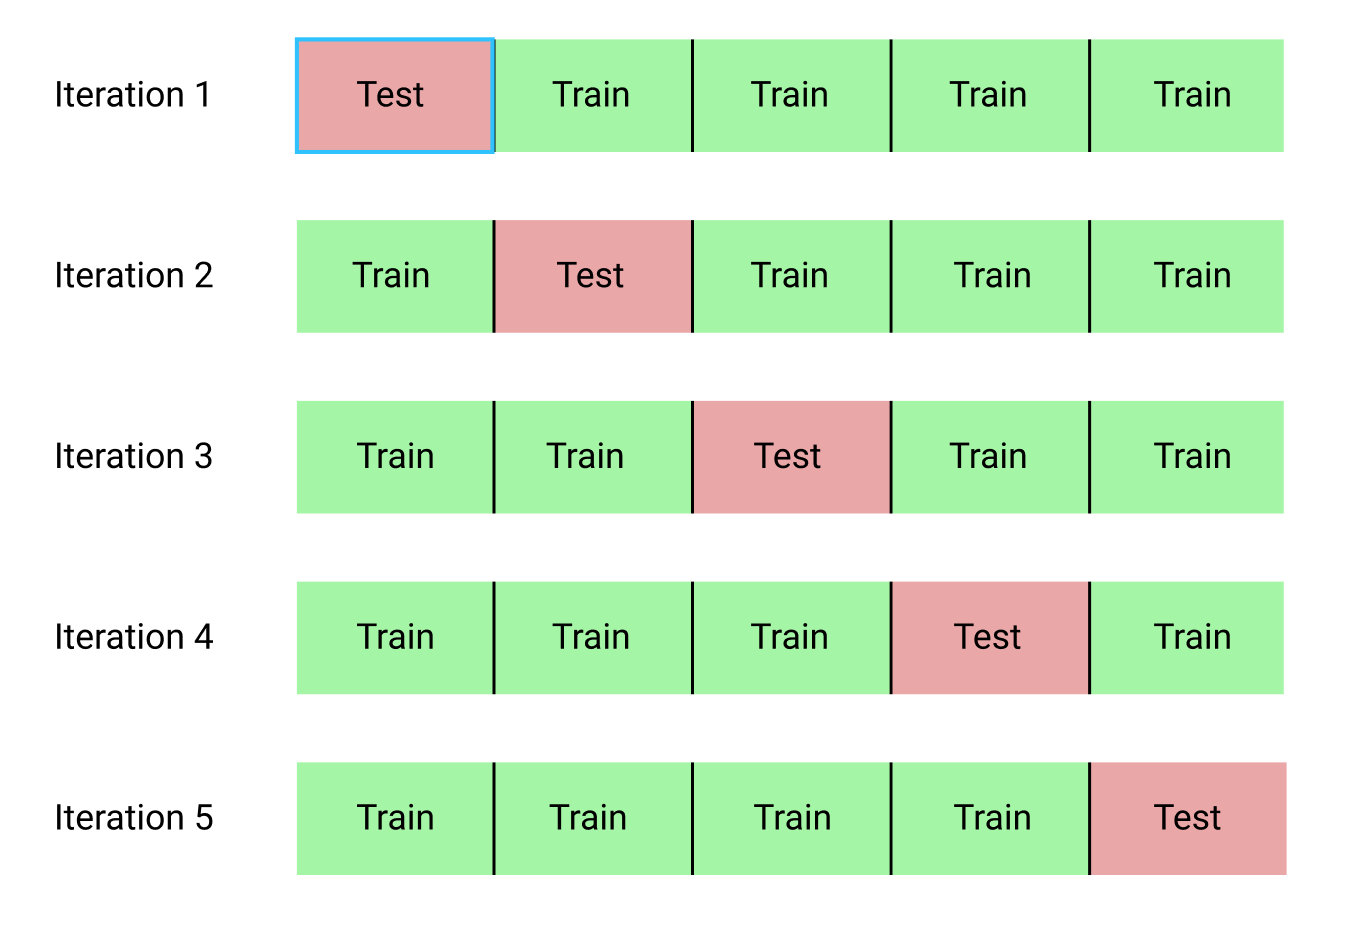
\includegraphics{img/kfold_cv.png}
\caption{title}
\end{figure}

    We selected 6 different hyperparameters to tune in the gradient boosting
regressor. These all will affect the model in different ways that are
hard to determine ahead of time, and the only method for finding the
best combination for a specific problem is to test them out! To read
about the hyperparameters, I suggest taking a look at the Scikit-Learn
documentation. For now, just know that we are trying to find the best
combination of hyperparameters and because there is no theory to tell us
which will work best, we just have to evaluate them, like runnning an
experiment!

In the code below, we create the Randomized Search Object passing in the
following parameters:

\begin{itemize}
\tightlist
\item
  estimator: the model
\item
  param\_distributions: the distribution of parameters we defined
\item
  cv the number of folds to use for k-fold cross validation
\item
  n\_iter: the number of different combinations to try
\item
  scoring: which metric to use when evaluating candidates
\item
  n\_jobs: number of cores to run in parallel (-1 will use all
  available)
\item
  verbose: how much information to display (1 displays a limited amount)
\item
  return\_train\_score: return the training score for each
  cross-validation fold
\item
  random\_state: fixes the random number generator used so we get the
  same results every run
\end{itemize}

The Randomized Search Object is trained the same way as any other
scikit-learn model. After training, we can compare all the different
hyperparameter combinations and find the best performing one.

    \begin{Verbatim}[commandchars=\\\{\}]
{\color{incolor}In [{\color{incolor}29}]:} \PY{c+c1}{\PYZsh{} Loss function to be optimized}
         \PY{n}{loss} \PY{o}{=} \PY{p}{[}\PY{l+s+s1}{\PYZsq{}}\PY{l+s+s1}{ls}\PY{l+s+s1}{\PYZsq{}}\PY{p}{,} \PY{l+s+s1}{\PYZsq{}}\PY{l+s+s1}{lad}\PY{l+s+s1}{\PYZsq{}}\PY{p}{,} \PY{l+s+s1}{\PYZsq{}}\PY{l+s+s1}{huber}\PY{l+s+s1}{\PYZsq{}}\PY{p}{]}
         
         \PY{c+c1}{\PYZsh{} Number of trees used in the boosting process}
         \PY{n}{n\PYZus{}estimators} \PY{o}{=} \PY{p}{[}\PY{l+m+mi}{100}\PY{p}{,} \PY{l+m+mi}{500}\PY{p}{,} \PY{l+m+mi}{900}\PY{p}{,} \PY{l+m+mi}{1100}\PY{p}{,} \PY{l+m+mi}{1500}\PY{p}{]}
         
         \PY{c+c1}{\PYZsh{} Maximum depth of each tree}
         \PY{n}{max\PYZus{}depth} \PY{o}{=} \PY{p}{[}\PY{l+m+mi}{2}\PY{p}{,} \PY{l+m+mi}{3}\PY{p}{,} \PY{l+m+mi}{5}\PY{p}{,} \PY{l+m+mi}{10}\PY{p}{,} \PY{l+m+mi}{15}\PY{p}{]}
         
         \PY{c+c1}{\PYZsh{} Minimum number of samples per leaf}
         \PY{n}{min\PYZus{}samples\PYZus{}leaf} \PY{o}{=} \PY{p}{[}\PY{l+m+mi}{1}\PY{p}{,} \PY{l+m+mi}{2}\PY{p}{,} \PY{l+m+mi}{4}\PY{p}{,} \PY{l+m+mi}{6}\PY{p}{,} \PY{l+m+mi}{8}\PY{p}{]}
         
         \PY{c+c1}{\PYZsh{} Minimum number of samples to split a node}
         \PY{n}{min\PYZus{}samples\PYZus{}split} \PY{o}{=} \PY{p}{[}\PY{l+m+mi}{2}\PY{p}{,} \PY{l+m+mi}{4}\PY{p}{,} \PY{l+m+mi}{6}\PY{p}{,} \PY{l+m+mi}{10}\PY{p}{]}
         
         \PY{c+c1}{\PYZsh{} Maximum number of features to consider for making splits}
         \PY{n}{max\PYZus{}features} \PY{o}{=} \PY{p}{[}\PY{l+s+s1}{\PYZsq{}}\PY{l+s+s1}{auto}\PY{l+s+s1}{\PYZsq{}}\PY{p}{,} \PY{l+s+s1}{\PYZsq{}}\PY{l+s+s1}{sqrt}\PY{l+s+s1}{\PYZsq{}}\PY{p}{,} \PY{l+s+s1}{\PYZsq{}}\PY{l+s+s1}{log2}\PY{l+s+s1}{\PYZsq{}}\PY{p}{,} \PY{k+kc}{None}\PY{p}{]}
         
         \PY{c+c1}{\PYZsh{} Define the grid of hyperparameters to search}
         \PY{n}{hyperparameter\PYZus{}grid} \PY{o}{=} \PY{p}{\PYZob{}}\PY{l+s+s1}{\PYZsq{}}\PY{l+s+s1}{loss}\PY{l+s+s1}{\PYZsq{}}\PY{p}{:} \PY{n}{loss}\PY{p}{,}
                                \PY{l+s+s1}{\PYZsq{}}\PY{l+s+s1}{n\PYZus{}estimators}\PY{l+s+s1}{\PYZsq{}}\PY{p}{:} \PY{n}{n\PYZus{}estimators}\PY{p}{,}
                                \PY{l+s+s1}{\PYZsq{}}\PY{l+s+s1}{max\PYZus{}depth}\PY{l+s+s1}{\PYZsq{}}\PY{p}{:} \PY{n}{max\PYZus{}depth}\PY{p}{,}
                                \PY{l+s+s1}{\PYZsq{}}\PY{l+s+s1}{min\PYZus{}samples\PYZus{}leaf}\PY{l+s+s1}{\PYZsq{}}\PY{p}{:} \PY{n}{min\PYZus{}samples\PYZus{}leaf}\PY{p}{,}
                                \PY{l+s+s1}{\PYZsq{}}\PY{l+s+s1}{min\PYZus{}samples\PYZus{}split}\PY{l+s+s1}{\PYZsq{}}\PY{p}{:} \PY{n}{min\PYZus{}samples\PYZus{}split}\PY{p}{,}
                                \PY{l+s+s1}{\PYZsq{}}\PY{l+s+s1}{max\PYZus{}features}\PY{l+s+s1}{\PYZsq{}}\PY{p}{:} \PY{n}{max\PYZus{}features}\PY{p}{\PYZcb{}}
\end{Verbatim}


    \begin{Verbatim}[commandchars=\\\{\}]
{\color{incolor}In [{\color{incolor}25}]:} \PY{c+c1}{\PYZsh{} Create the model to use for hyperparameter tuning}
         \PY{n}{model} \PY{o}{=} \PY{n}{GradientBoostingRegressor}\PY{p}{(}\PY{n}{random\PYZus{}state} \PY{o}{=} \PY{l+m+mi}{42}\PY{p}{)}
         
         \PY{c+c1}{\PYZsh{} Set up the random search with 4\PYZhy{}fold cross validation}
         \PY{n}{random\PYZus{}cv} \PY{o}{=} \PY{n}{RandomizedSearchCV}\PY{p}{(}\PY{n}{estimator}\PY{o}{=}\PY{n}{model}\PY{p}{,}
                                        \PY{n}{param\PYZus{}distributions}\PY{o}{=}\PY{n}{hyperparameter\PYZus{}grid}\PY{p}{,}
                                        \PY{n}{cv}\PY{o}{=}\PY{l+m+mi}{4}\PY{p}{,} \PY{n}{n\PYZus{}iter}\PY{o}{=}\PY{l+m+mi}{25}\PY{p}{,} 
                                        \PY{n}{scoring} \PY{o}{=} \PY{l+s+s1}{\PYZsq{}}\PY{l+s+s1}{neg\PYZus{}mean\PYZus{}absolute\PYZus{}error}\PY{l+s+s1}{\PYZsq{}}\PY{p}{,}
                                        \PY{n}{n\PYZus{}jobs} \PY{o}{=} \PY{o}{\PYZhy{}}\PY{l+m+mi}{1}\PY{p}{,} \PY{n}{verbose} \PY{o}{=} \PY{l+m+mi}{1}\PY{p}{,} 
                                        \PY{n}{return\PYZus{}train\PYZus{}score} \PY{o}{=} \PY{k+kc}{True}\PY{p}{,}
                                        \PY{n}{random\PYZus{}state}\PY{o}{=}\PY{l+m+mi}{42}\PY{p}{)}
\end{Verbatim}


    Using random search is a good method to narrow down the possible
hyperparameters to try. Initially, we had no idea which combination
would work the best, but this at least narrows down the range of
options.

We could use the random search results to inform a grid search by
creating a grid with hyperparameters close to those that worked best
during the randomized search. However, rather than evaluating all of
these settings again, I will focus on a single one, the number of trees
in the forest (n\_estimators). By varying only one hyperparameter, we
can directly observe how it affects performance. In the case of the
number of trees, we would expect to see a significant affect on the
amount of under vs overfitting.

Here we will use grid search with a grid that only has the n\_estimators
hyperparameter. We will evaluate a range of trees then plot the training
and testing performance to get an idea of what increasing the number of
trees does for our model. We will fix the other hyperparameters at the
best values returned from random search to isolate the number of trees
effect.

    \begin{Verbatim}[commandchars=\\\{\}]
{\color{incolor}In [{\color{incolor}22}]:} \PY{c+c1}{\PYZsh{} Fit on the training data}
         \PY{n}{random\PYZus{}cv}\PY{o}{.}\PY{n}{fit}\PY{p}{(}\PY{n}{X}\PY{p}{,} \PY{n}{y}\PY{p}{)}
\end{Verbatim}


    \begin{Verbatim}[commandchars=\\\{\}]
Fitting 4 folds for each of 25 candidates, totalling 100 fits

    \end{Verbatim}

    \begin{Verbatim}[commandchars=\\\{\}]
[Parallel(n\_jobs=-1)]: Done  42 tasks      | elapsed: 136.3min
[Parallel(n\_jobs=-1)]: Done 100 out of 100 | elapsed: 254.4min finished

    \end{Verbatim}

\begin{Verbatim}[commandchars=\\\{\}]
{\color{outcolor}Out[{\color{outcolor}22}]:} RandomizedSearchCV(cv=4, error\_score='raise',
                   estimator=GradientBoostingRegressor(alpha=0.9, criterion='friedman\_mse', init=None,
                      learning\_rate=0.1, loss='ls', max\_depth=3, max\_features=None,
                      max\_leaf\_nodes=None, min\_impurity\_decrease=0.0,
                      min\_impurity\_split=None, min\_samples\_leaf=1,
                      min\_samples\_split=2, min\_weight\_fraction\_leaf=0.0,
                      n\_estimators=100, presort='auto', random\_state=42,
                      subsample=1.0, verbose=0, warm\_start=False),
                   fit\_params=None, iid=True, n\_iter=25, n\_jobs=-1,
                   param\_distributions=\{'loss': ['ls', 'lad', 'huber'], 'n\_estimators': [100, 500, 900, 1100, 1500], 'max\_depth': [2, 3, 5, 10, 15], 'min\_samples\_leaf': [1, 2, 4, 6, 8], 'min\_samples\_split': [2, 4, 6, 10], 'max\_features': ['auto', 'sqrt', 'log2', None]\},
                   pre\_dispatch='2*n\_jobs', random\_state=42, refit=True,
                   return\_train\_score=True, scoring='neg\_mean\_absolute\_error',
                   verbose=1)
\end{Verbatim}
            
    \begin{Verbatim}[commandchars=\\\{\}]
{\color{incolor}In [{\color{incolor}23}]:} \PY{c+c1}{\PYZsh{} Get all of the cv results and sort by the test performance}
         \PY{n}{random\PYZus{}results} \PY{o}{=} \PY{n}{pd}\PY{o}{.}\PY{n}{DataFrame}\PY{p}{(}\PY{n}{random\PYZus{}cv}\PY{o}{.}\PY{n}{cv\PYZus{}results\PYZus{}}\PY{p}{)}\PY{o}{.}\PY{n}{sort\PYZus{}values}\PY{p}{(}\PY{l+s+s1}{\PYZsq{}}\PY{l+s+s1}{mean\PYZus{}test\PYZus{}score}\PY{l+s+s1}{\PYZsq{}}\PY{p}{,} \PY{n}{ascending} \PY{o}{=} \PY{k+kc}{False}\PY{p}{)}
         
         \PY{n}{random\PYZus{}results}\PY{o}{.}\PY{n}{head}\PY{p}{(}\PY{l+m+mi}{10}\PY{p}{)}
\end{Verbatim}


\begin{Verbatim}[commandchars=\\\{\}]
{\color{outcolor}Out[{\color{outcolor}23}]:}     mean\_fit\_time  std\_fit\_time  mean\_score\_time  std\_score\_time  \textbackslash{}
         18    2507.848624     33.300083         1.114147        0.046026   
         6     2334.942136     14.048862         3.983173        0.178638   
         10    2124.735126     16.437696         1.522919        0.124221   
         2     1126.109925     11.526923         0.729106        0.022121   
         8      816.886923      2.946848         2.328359        0.080240   
         4      607.912191     16.881561         1.617521        0.020844   
         15     444.175597     11.911947         0.252447        0.019988   
         12     417.570377      6.769207         0.562246        0.038942   
         20     277.970365      1.312068         0.769979        0.024256   
         19     544.968845     13.669563         1.048108        0.075696   
         
            param\_n\_estimators param\_min\_samples\_split param\_min\_samples\_leaf  \textbackslash{}
         18                500                       6                      1   
         6                1500                       6                      2   
         10               1100                      10                      6   
         2                 500                       4                      2   
         8                1500                       6                      2   
         4                 900                       6                      6   
         15                100                       4                      8   
         12                500                       6                      6   
         20                500                       6                      1   
         19               1100                       6                      2   
         
            param\_max\_features param\_max\_depth param\_loss  \textbackslash{}
         18               auto              15      huber   
         6                sqrt              15      huber   
         10               None              10      huber   
         2                auto              10      huber   
         8                sqrt              10      huber   
         4                sqrt              15        lad   
         15               auto              15         ls   
         12               None               5        lad   
         20               sqrt              10      huber   
         19               auto               3        lad   
         
                                                        params  split0\_test\_score  \textbackslash{}
         18  \{'n\_estimators': 500, 'min\_samples\_split': 6, {\ldots}         -12.305691   
         6   \{'n\_estimators': 1500, 'min\_samples\_split': 6,{\ldots}         -12.627793   
         10  \{'n\_estimators': 1100, 'min\_samples\_split': 10{\ldots}         -12.673745   
         2   \{'n\_estimators': 500, 'min\_samples\_split': 4, {\ldots}         -12.787344   
         8   \{'n\_estimators': 1500, 'min\_samples\_split': 6,{\ldots}         -12.850447   
         4   \{'n\_estimators': 900, 'min\_samples\_split': 6, {\ldots}         -13.090788   
         15  \{'n\_estimators': 100, 'min\_samples\_split': 4, {\ldots}         -12.971418   
         12  \{'n\_estimators': 500, 'min\_samples\_split': 6, {\ldots}         -13.133786   
         20  \{'n\_estimators': 500, 'min\_samples\_split': 6, {\ldots}         -13.177236   
         19  \{'n\_estimators': 1100, 'min\_samples\_split': 6,{\ldots}         -13.386209   
         
             split1\_test\_score  split2\_test\_score  split3\_test\_score  mean\_test\_score  \textbackslash{}
         18         -12.479495         -12.442696         -12.427981       -12.413966   
         6          -12.698014         -12.631877         -12.683700       -12.660346   
         10         -12.856237         -12.723406         -12.745506       -12.749723   
         2          -13.013390         -12.868137         -12.835454       -12.876082   
         8          -12.915562         -12.861111         -12.910616       -12.884434   
         4          -13.138139         -13.083387         -13.114572       -13.106721   
         15         -13.133815         -13.147728         -13.187837       -13.110199   
         12         -13.354358         -13.123513         -13.193716       -13.201344   
         20         -13.351234         -13.204357         -13.226549       -13.239844   
         19         -13.603856         -13.359980         -13.449208       -13.449813   
         
             std\_test\_score  rank\_test\_score  split0\_train\_score  split1\_train\_score  \textbackslash{}
         18        0.065268                1           -0.520493           -0.594302   
         6         0.030961                2           -0.169508           -0.182260   
         10        0.066762                3           -4.092415           -3.991364   
         2         0.084324                4           -4.687187           -4.837749   
         8         0.028955                5           -2.252518           -2.239778   
         4         0.021489                6           -6.522978           -6.167718   
         15        0.082544                7           -5.671360           -5.682671   
         12        0.092322                8          -12.295324          -12.235389   
         20        0.066641                9           -5.800267           -5.828240   
         19        0.094665               10          -13.198940          -13.122769   
         
             split2\_train\_score  split3\_train\_score  mean\_train\_score  std\_train\_score  
         18           -0.559897           -0.576908         -0.562900         0.027339  
         6            -0.178315           -0.178455         -0.177134         0.004679  
         10           -4.054033           -3.739914         -3.969431         0.137333  
         2            -4.636145           -4.898625         -4.764926         0.107012  
         8            -2.243961           -2.234976         -2.242808         0.006445  
         4            -6.300072           -6.460923         -6.362923         0.138994  
         15           -5.853450           -5.688289         -5.723943         0.075019  
         12          -12.273618          -12.294744        -12.274769         0.024360  
         20           -5.721568           -5.737856         -5.771983         0.043793  
         19          -13.188596          -13.171312        -13.170404         0.029220  
\end{Verbatim}
            
    \begin{Verbatim}[commandchars=\\\{\}]
{\color{incolor}In [{\color{incolor}24}]:} \PY{n}{random\PYZus{}cv}\PY{o}{.}\PY{n}{best\PYZus{}estimator\PYZus{}}
\end{Verbatim}


\begin{Verbatim}[commandchars=\\\{\}]
{\color{outcolor}Out[{\color{outcolor}24}]:} GradientBoostingRegressor(alpha=0.9, criterion='friedman\_mse', init=None,
                      learning\_rate=0.1, loss='huber', max\_depth=15,
                      max\_features='auto', max\_leaf\_nodes=None,
                      min\_impurity\_decrease=0.0, min\_impurity\_split=None,
                      min\_samples\_leaf=1, min\_samples\_split=6,
                      min\_weight\_fraction\_leaf=0.0, n\_estimators=500,
                      presort='auto', random\_state=42, subsample=1.0, verbose=0,
                      warm\_start=False)
\end{Verbatim}
            
    \begin{Verbatim}[commandchars=\\\{\}]
{\color{incolor}In [{\color{incolor}33}]:} \PY{c+c1}{\PYZsh{} Number of trees used in the boosting process}
         \PY{n}{n\PYZus{}estimators} \PY{o}{=} \PY{p}{[}\PY{l+m+mi}{100}\PY{p}{,} \PY{l+m+mi}{500}\PY{p}{,} \PY{l+m+mi}{900}\PY{p}{,} \PY{l+m+mi}{1100}\PY{p}{,} \PY{l+m+mi}{1500}\PY{p}{]}
         
         \PY{c+c1}{\PYZsh{} Maximum depth of each tree}
         \PY{n}{max\PYZus{}depth} \PY{o}{=} \PY{p}{[}\PY{l+m+mi}{2}\PY{p}{,} \PY{l+m+mi}{3}\PY{p}{,} \PY{l+m+mi}{5}\PY{p}{,} \PY{l+m+mi}{10}\PY{p}{,} \PY{l+m+mi}{15}\PY{p}{]}
         
         \PY{c+c1}{\PYZsh{} Minimum number of samples per leaf}
         \PY{n}{min\PYZus{}samples\PYZus{}leaf} \PY{o}{=} \PY{p}{[}\PY{l+m+mi}{1}\PY{p}{,} \PY{l+m+mi}{2}\PY{p}{,} \PY{l+m+mi}{4}\PY{p}{,} \PY{l+m+mi}{6}\PY{p}{,} \PY{l+m+mi}{8}\PY{p}{]}
         
         \PY{c+c1}{\PYZsh{} Minimum number of samples to split a node}
         \PY{n}{min\PYZus{}samples\PYZus{}split} \PY{o}{=} \PY{p}{[}\PY{l+m+mi}{2}\PY{p}{,} \PY{l+m+mi}{4}\PY{p}{,} \PY{l+m+mi}{6}\PY{p}{,} \PY{l+m+mi}{10}\PY{p}{]}
         
         \PY{c+c1}{\PYZsh{} Maximum number of features to consider for making splits}
         \PY{n}{max\PYZus{}features} \PY{o}{=} \PY{p}{[}\PY{l+s+s1}{\PYZsq{}}\PY{l+s+s1}{auto}\PY{l+s+s1}{\PYZsq{}}\PY{p}{,} \PY{l+s+s1}{\PYZsq{}}\PY{l+s+s1}{sqrt}\PY{l+s+s1}{\PYZsq{}}\PY{p}{,} \PY{l+s+s1}{\PYZsq{}}\PY{l+s+s1}{log2}\PY{l+s+s1}{\PYZsq{}}\PY{p}{,} \PY{k+kc}{None}\PY{p}{]}
         
         \PY{c+c1}{\PYZsh{} Define the grid of hyperparameters to search}
         \PY{n}{hyperparameter\PYZus{}gridr} \PY{o}{=} \PY{p}{\PYZob{}}\PY{l+s+s1}{\PYZsq{}}\PY{l+s+s1}{n\PYZus{}estimators}\PY{l+s+s1}{\PYZsq{}}\PY{p}{:} \PY{n}{n\PYZus{}estimators}\PY{p}{,}
                                \PY{l+s+s1}{\PYZsq{}}\PY{l+s+s1}{max\PYZus{}depth}\PY{l+s+s1}{\PYZsq{}}\PY{p}{:} \PY{n}{max\PYZus{}depth}\PY{p}{,}
                                \PY{l+s+s1}{\PYZsq{}}\PY{l+s+s1}{min\PYZus{}samples\PYZus{}leaf}\PY{l+s+s1}{\PYZsq{}}\PY{p}{:} \PY{n}{min\PYZus{}samples\PYZus{}leaf}\PY{p}{,}
                                \PY{l+s+s1}{\PYZsq{}}\PY{l+s+s1}{min\PYZus{}samples\PYZus{}split}\PY{l+s+s1}{\PYZsq{}}\PY{p}{:} \PY{n}{min\PYZus{}samples\PYZus{}split}\PY{p}{,}
                                \PY{l+s+s1}{\PYZsq{}}\PY{l+s+s1}{max\PYZus{}features}\PY{l+s+s1}{\PYZsq{}}\PY{p}{:} \PY{n}{max\PYZus{}features}\PY{p}{\PYZcb{}}
\end{Verbatim}


    \begin{Verbatim}[commandchars=\\\{\}]
{\color{incolor}In [{\color{incolor}34}]:} \PY{c+c1}{\PYZsh{} Create the model to use for hyperparameter tuning}
         \PY{n}{model\PYZus{}r} \PY{o}{=} \PY{n}{RandomForestRegressor}\PY{p}{(}\PY{n}{random\PYZus{}state} \PY{o}{=} \PY{l+m+mi}{42}\PY{p}{)}
         
         \PY{c+c1}{\PYZsh{} Set up the random search with 4\PYZhy{}fold cross validation}
         \PY{n}{random\PYZus{}cv\PYZus{}r} \PY{o}{=} \PY{n}{RandomizedSearchCV}\PY{p}{(}\PY{n}{estimator}\PY{o}{=}\PY{n}{model}\PY{p}{,}
                                        \PY{n}{param\PYZus{}distributions}\PY{o}{=}\PY{n}{hyperparameter\PYZus{}gridr}\PY{p}{,}
                                        \PY{n}{cv}\PY{o}{=}\PY{l+m+mi}{4}\PY{p}{,} \PY{n}{n\PYZus{}iter}\PY{o}{=}\PY{l+m+mi}{25}\PY{p}{,} 
                                        \PY{n}{scoring} \PY{o}{=} \PY{l+s+s1}{\PYZsq{}}\PY{l+s+s1}{neg\PYZus{}mean\PYZus{}absolute\PYZus{}error}\PY{l+s+s1}{\PYZsq{}}\PY{p}{,}
                                        \PY{n}{n\PYZus{}jobs} \PY{o}{=} \PY{o}{\PYZhy{}}\PY{l+m+mi}{1}\PY{p}{,} \PY{n}{verbose} \PY{o}{=} \PY{l+m+mi}{1}\PY{p}{,} 
                                        \PY{n}{return\PYZus{}train\PYZus{}score} \PY{o}{=} \PY{k+kc}{True}\PY{p}{,}
                                        \PY{n}{random\PYZus{}state}\PY{o}{=}\PY{l+m+mi}{42}\PY{p}{)}
\end{Verbatim}


    \begin{Verbatim}[commandchars=\\\{\}]
{\color{incolor}In [{\color{incolor}35}]:} \PY{c+c1}{\PYZsh{} Fit on the training data}
         \PY{n}{random\PYZus{}cv\PYZus{}r}\PY{o}{.}\PY{n}{fit}\PY{p}{(}\PY{n}{X}\PY{p}{,} \PY{n}{y}\PY{p}{)}
\end{Verbatim}


    \begin{Verbatim}[commandchars=\\\{\}]
Fitting 4 folds for each of 25 candidates, totalling 100 fits

    \end{Verbatim}

    \begin{Verbatim}[commandchars=\\\{\}]
[Parallel(n\_jobs=-1)]: Done  42 tasks      | elapsed: 34.8min
[Parallel(n\_jobs=-1)]: Done 100 out of 100 | elapsed: 100.7min finished

    \end{Verbatim}

\begin{Verbatim}[commandchars=\\\{\}]
{\color{outcolor}Out[{\color{outcolor}35}]:} RandomizedSearchCV(cv=4, error\_score='raise',
                   estimator=RandomForestRegressor(bootstrap=True, criterion='mse', max\_depth=None,
                    max\_features='auto', max\_leaf\_nodes=None,
                    min\_impurity\_decrease=0.0, min\_impurity\_split=None,
                    min\_samples\_leaf=1, min\_samples\_split=2,
                    min\_weight\_fraction\_leaf=0.0, n\_estimators=10, n\_jobs=1,
                    oob\_score=False, random\_state=42, verbose=0, warm\_start=False),
                   fit\_params=None, iid=True, n\_iter=25, n\_jobs=-1,
                   param\_distributions=\{'n\_estimators': [100, 500, 900, 1100, 1500], 'max\_depth': [2, 3, 5, 10, 15], 'min\_samples\_leaf': [1, 2, 4, 6, 8], 'min\_samples\_split': [2, 4, 6, 10], 'max\_features': ['auto', 'sqrt', 'log2', None]\},
                   pre\_dispatch='2*n\_jobs', random\_state=42, refit=True,
                   return\_train\_score=True, scoring='neg\_mean\_absolute\_error',
                   verbose=1)
\end{Verbatim}
            
    \begin{Verbatim}[commandchars=\\\{\}]
{\color{incolor}In [{\color{incolor}36}]:} \PY{c+c1}{\PYZsh{} Get all of the cv results and sort by the test performance}
         \PY{n}{random\PYZus{}results\PYZus{}r} \PY{o}{=} \PY{n}{pd}\PY{o}{.}\PY{n}{DataFrame}\PY{p}{(}\PY{n}{random\PYZus{}cv\PYZus{}r}\PY{o}{.}\PY{n}{cv\PYZus{}results\PYZus{}}\PY{p}{)}\PY{o}{.}\PY{n}{sort\PYZus{}values}\PY{p}{(}\PY{l+s+s1}{\PYZsq{}}\PY{l+s+s1}{mean\PYZus{}test\PYZus{}score}\PY{l+s+s1}{\PYZsq{}}\PY{p}{,} \PY{n}{ascending} \PY{o}{=} \PY{k+kc}{False}\PY{p}{)}
         
         \PY{n}{random\PYZus{}results\PYZus{}r}\PY{o}{.}\PY{n}{head}\PY{p}{(}\PY{l+m+mi}{10}\PY{p}{)}
\end{Verbatim}


\begin{Verbatim}[commandchars=\\\{\}]
{\color{outcolor}Out[{\color{outcolor}36}]:}     mean\_fit\_time  std\_fit\_time  mean\_score\_time  std\_score\_time  \textbackslash{}
         24     654.204295      0.891554         3.729978        0.300693   
         18     317.750335      0.756234         1.705690        0.019739   
         21     977.692213      1.950855         5.938960        0.255091   
         22     337.716268      1.645129         1.978627        0.135513   
         4      775.745531      1.269862         3.482658        0.025827   
         5      566.171118      1.887277         2.433663        0.078843   
         11     484.249159      0.857920         2.128310        0.032508   
         7       65.005917      0.268167         1.639223        0.047122   
         19     106.013270      0.335120         2.741918        0.063613   
         0       12.197284      0.061941         0.353054        0.024050   
         
            param\_n\_estimators param\_min\_samples\_split param\_min\_samples\_leaf  \textbackslash{}
         24                900                       2                      2   
         18                500                       4                      4   
         21               1500                       2                      6   
         22                500                       2                      8   
         4                1500                       4                      8   
         5                1100                       6                      6   
         11                900                       6                      8   
         7                 500                       6                      2   
         19                900                       6                      4   
         0                 100                       2                      6   
         
            param\_max\_features param\_max\_depth  \textbackslash{}
         24               None              15   
         18               auto              15   
         21               auto              15   
         22               None              15   
         4                auto              10   
         5                auto              10   
         11               auto              10   
         7                sqrt              15   
         19               log2              15   
         0                log2              15   
         
                                                        params  split0\_test\_score  \textbackslash{}
         24  \{'n\_estimators': 900, 'min\_samples\_split': 2, {\ldots}         -13.402021   
         18  \{'n\_estimators': 500, 'min\_samples\_split': 4, {\ldots}         -13.464452   
         21  \{'n\_estimators': 1500, 'min\_samples\_split': 2,{\ldots}         -13.523780   
         22  \{'n\_estimators': 500, 'min\_samples\_split': 2, {\ldots}         -13.582721   
         4   \{'n\_estimators': 1500, 'min\_samples\_split': 4,{\ldots}         -14.077486   
         5   \{'n\_estimators': 1100, 'min\_samples\_split': 6,{\ldots}         -14.075185   
         11  \{'n\_estimators': 900, 'min\_samples\_split': 6, {\ldots}         -14.080369   
         7   \{'n\_estimators': 500, 'min\_samples\_split': 6, {\ldots}         -14.974741   
         19  \{'n\_estimators': 900, 'min\_samples\_split': 6, {\ldots}         -15.310081   
         0   \{'n\_estimators': 100, 'min\_samples\_split': 2, {\ldots}         -15.361428   
         
             split1\_test\_score  split2\_test\_score  split3\_test\_score  mean\_test\_score  \textbackslash{}
         24         -13.554404         -13.410878         -13.519550       -13.471712   
         18         -13.606978         -13.457409         -13.578375       -13.526802   
         21         -13.666443         -13.509659         -13.623440       -13.580830   
         22         -13.714271         -13.552559         -13.674083       -13.630908   
         4          -14.215993         -14.012058         -14.188323       -14.123464   
         5          -14.216376         -14.013973         -14.188940       -14.123618   
         11         -14.215481         -14.011806         -14.190598       -14.124562   
         7          -15.099844         -14.904913         -15.098282       -15.019444   
         19         -15.402012         -15.248064         -15.392534       -15.338172   
         0          -15.442778         -15.282314         -15.432247       -15.379691   
         
             std\_test\_score  rank\_test\_score  split0\_train\_score  split1\_train\_score  \textbackslash{}
         24        0.066491                1          -10.033439           -9.918535   
         18        0.066691                2          -10.492844          -10.387390   
         21        0.066078                3          -10.949502          -10.859095   
         22        0.065715                4          -11.318162          -11.223526   
         4         0.082604                5          -13.212488          -13.138087   
         5         0.082521                6          -13.161659          -13.086809   
         11        0.082605                7          -13.211491          -13.137699   
         7         0.083360                8          -13.287991          -13.215743   
         19        0.063126                9          -14.160627          -14.061115   
         0         0.064339               10          -14.391767          -14.303452   
         
             split2\_train\_score  split3\_train\_score  mean\_train\_score  std\_train\_score  
         24           -9.997933          -10.048048         -9.999489         0.050166  
         18          -10.454143          -10.490489        -10.456217         0.042596  
         21          -10.909222          -10.931594        -10.912353         0.033899  
         22          -11.275046          -11.299287        -11.279005         0.035490  
         4           -13.225316          -13.235104        -13.202749         0.038184  
         5           -13.179024          -13.186117        -13.153402         0.039464  
         11          -13.226023          -13.238274        -13.203372         0.039083  
         7           -13.255517          -13.266233        -13.256371         0.026213  
         19          -14.165509          -14.104802        -14.123013         0.042964  
         0           -14.408617          -14.329578        -14.358353         0.043258  
\end{Verbatim}
            
    \begin{Verbatim}[commandchars=\\\{\}]
{\color{incolor}In [{\color{incolor}14}]:} \PY{c+c1}{\PYZsh{} Create a range of trees to evaluate}
         \PY{n}{trees\PYZus{}grid} \PY{o}{=} \PY{p}{\PYZob{}}\PY{l+s+s1}{\PYZsq{}}\PY{l+s+s1}{n\PYZus{}estimators}\PY{l+s+s1}{\PYZsq{}}\PY{p}{:} \PY{p}{[}\PY{l+m+mi}{100}\PY{p}{,} \PY{l+m+mi}{150}\PY{p}{,} \PY{l+m+mi}{200}\PY{p}{,} \PY{l+m+mi}{250}\PY{p}{,} \PY{l+m+mi}{300}\PY{p}{,} \PY{l+m+mi}{350}\PY{p}{,} \PY{l+m+mi}{400}\PY{p}{,} \PY{l+m+mi}{450}\PY{p}{,} \PY{l+m+mi}{500}\PY{p}{,} \PY{l+m+mi}{550}\PY{p}{,} \PY{l+m+mi}{600}\PY{p}{,} \PY{l+m+mi}{650}\PY{p}{,} \PY{l+m+mi}{700}\PY{p}{,} \PY{l+m+mi}{750}\PY{p}{,} \PY{l+m+mi}{800}\PY{p}{]}\PY{p}{\PYZcb{}}
         
         \PY{n}{model} \PY{o}{=} \PY{n}{GradientBoostingRegressor}\PY{p}{(}\PY{n}{alpha}\PY{o}{=}\PY{l+m+mf}{0.9}\PY{p}{,} \PY{n}{criterion}\PY{o}{=}\PY{l+s+s1}{\PYZsq{}}\PY{l+s+s1}{friedman\PYZus{}mse}\PY{l+s+s1}{\PYZsq{}}\PY{p}{,} \PY{n}{init}\PY{o}{=}\PY{k+kc}{None}\PY{p}{,}
                      \PY{n}{learning\PYZus{}rate}\PY{o}{=}\PY{l+m+mf}{0.1}\PY{p}{,} \PY{n}{loss}\PY{o}{=}\PY{l+s+s1}{\PYZsq{}}\PY{l+s+s1}{huber}\PY{l+s+s1}{\PYZsq{}}\PY{p}{,} \PY{n}{max\PYZus{}depth}\PY{o}{=}\PY{l+m+mi}{15}\PY{p}{,}
                      \PY{n}{max\PYZus{}features}\PY{o}{=}\PY{l+s+s1}{\PYZsq{}}\PY{l+s+s1}{auto}\PY{l+s+s1}{\PYZsq{}}\PY{p}{,} \PY{n}{max\PYZus{}leaf\PYZus{}nodes}\PY{o}{=}\PY{k+kc}{None}\PY{p}{,}
                      \PY{n}{min\PYZus{}impurity\PYZus{}decrease}\PY{o}{=}\PY{l+m+mf}{0.0}\PY{p}{,} \PY{n}{min\PYZus{}impurity\PYZus{}split}\PY{o}{=}\PY{k+kc}{None}\PY{p}{,}
                      \PY{n}{min\PYZus{}samples\PYZus{}leaf}\PY{o}{=}\PY{l+m+mi}{1}\PY{p}{,} \PY{n}{min\PYZus{}samples\PYZus{}split}\PY{o}{=}\PY{l+m+mi}{6}\PY{p}{,}
                      \PY{n}{min\PYZus{}weight\PYZus{}fraction\PYZus{}leaf}\PY{o}{=}\PY{l+m+mf}{0.0}\PY{p}{,} \PY{n}{n\PYZus{}estimators}\PY{o}{=}\PY{l+m+mi}{500}\PY{p}{,}
                      \PY{n}{presort}\PY{o}{=}\PY{l+s+s1}{\PYZsq{}}\PY{l+s+s1}{auto}\PY{l+s+s1}{\PYZsq{}}\PY{p}{,} \PY{n}{random\PYZus{}state}\PY{o}{=}\PY{l+m+mi}{42}\PY{p}{,} \PY{n}{subsample}\PY{o}{=}\PY{l+m+mf}{1.0}\PY{p}{,} \PY{n}{verbose}\PY{o}{=}\PY{l+m+mi}{0}\PY{p}{,}
                      \PY{n}{warm\PYZus{}start}\PY{o}{=}\PY{k+kc}{False}\PY{p}{)}
         
         \PY{c+c1}{\PYZsh{} Grid Search Object using the trees range and the random forest model}
         \PY{n}{grid\PYZus{}search} \PY{o}{=} \PY{n}{GridSearchCV}\PY{p}{(}\PY{n}{estimator} \PY{o}{=} \PY{n}{model}\PY{p}{,} \PY{n}{param\PYZus{}grid}\PY{o}{=}\PY{n}{trees\PYZus{}grid}\PY{p}{,} \PY{n}{cv} \PY{o}{=} \PY{l+m+mi}{4}\PY{p}{,} 
                                    \PY{n}{scoring} \PY{o}{=} \PY{l+s+s1}{\PYZsq{}}\PY{l+s+s1}{neg\PYZus{}mean\PYZus{}absolute\PYZus{}error}\PY{l+s+s1}{\PYZsq{}}\PY{p}{,} \PY{n}{verbose} \PY{o}{=} \PY{l+m+mi}{1}\PY{p}{,}
                                    \PY{n}{n\PYZus{}jobs} \PY{o}{=} \PY{o}{\PYZhy{}}\PY{l+m+mi}{1}\PY{p}{,} \PY{n}{return\PYZus{}train\PYZus{}score} \PY{o}{=} \PY{k+kc}{True}\PY{p}{)}
\end{Verbatim}


    \begin{Verbatim}[commandchars=\\\{\}]
{\color{incolor}In [{\color{incolor}15}]:} \PY{c+c1}{\PYZsh{} Fit the grid search}
         \PY{n}{grid\PYZus{}search}\PY{o}{.}\PY{n}{fit}\PY{p}{(}\PY{n}{X}\PY{p}{,} \PY{n}{y}\PY{p}{)}
\end{Verbatim}


    \begin{Verbatim}[commandchars=\\\{\}]
Fitting 4 folds for each of 15 candidates, totalling 60 fits

    \end{Verbatim}

    \begin{Verbatim}[commandchars=\\\{\}]
[Parallel(n\_jobs=-1)]: Done  42 tasks      | elapsed: 355.5min
[Parallel(n\_jobs=-1)]: Done  60 out of  60 | elapsed: 606.7min finished

    \end{Verbatim}

\begin{Verbatim}[commandchars=\\\{\}]
{\color{outcolor}Out[{\color{outcolor}15}]:} GridSearchCV(cv=4, error\_score='raise',
                estimator=GradientBoostingRegressor(alpha=0.9, criterion='friedman\_mse', init=None,
                      learning\_rate=0.1, loss='huber', max\_depth=15,
                      max\_features='auto', max\_leaf\_nodes=None,
                      min\_impurity\_decrease=0.0, min\_impurity\_split=None,
                      min\_samples\_leaf=1, min\_samples\_split=6,
                      min\_weight\_fraction\_leaf=0.0, n\_estimators=500,
                      presort='auto', random\_state=42, subsample=1.0, verbose=0,
                      warm\_start=False),
                fit\_params=None, iid=True, n\_jobs=-1,
                param\_grid=\{'n\_estimators': [100, 150, 200, 250, 300, 350, 400, 450, 500, 550, 600, 650, 700, 750, 800]\},
                pre\_dispatch='2*n\_jobs', refit=True, return\_train\_score=True,
                scoring='neg\_mean\_absolute\_error', verbose=1)
\end{Verbatim}
            
    \begin{Verbatim}[commandchars=\\\{\}]
{\color{incolor}In [{\color{incolor}16}]:} \PY{c+c1}{\PYZsh{} Get the results into a dataframe}
         \PY{n}{results} \PY{o}{=} \PY{n}{pd}\PY{o}{.}\PY{n}{DataFrame}\PY{p}{(}\PY{n}{grid\PYZus{}search}\PY{o}{.}\PY{n}{cv\PYZus{}results\PYZus{}}\PY{p}{)}
         
         \PY{c+c1}{\PYZsh{} Plot the training and testing error vs number of trees}
         \PY{n}{figsize}\PY{p}{(}\PY{l+m+mi}{8}\PY{p}{,} \PY{l+m+mi}{8}\PY{p}{)}
         \PY{n}{plt}\PY{o}{.}\PY{n}{style}\PY{o}{.}\PY{n}{use}\PY{p}{(}\PY{l+s+s1}{\PYZsq{}}\PY{l+s+s1}{fivethirtyeight}\PY{l+s+s1}{\PYZsq{}}\PY{p}{)}
         \PY{n}{plt}\PY{o}{.}\PY{n}{plot}\PY{p}{(}\PY{n}{results}\PY{p}{[}\PY{l+s+s1}{\PYZsq{}}\PY{l+s+s1}{param\PYZus{}n\PYZus{}estimators}\PY{l+s+s1}{\PYZsq{}}\PY{p}{]}\PY{p}{,} \PY{o}{\PYZhy{}}\PY{l+m+mi}{1} \PY{o}{*} \PY{n}{results}\PY{p}{[}\PY{l+s+s1}{\PYZsq{}}\PY{l+s+s1}{mean\PYZus{}test\PYZus{}score}\PY{l+s+s1}{\PYZsq{}}\PY{p}{]}\PY{p}{,} \PY{n}{label} \PY{o}{=} \PY{l+s+s1}{\PYZsq{}}\PY{l+s+s1}{Testing Error}\PY{l+s+s1}{\PYZsq{}}\PY{p}{)}
         \PY{n}{plt}\PY{o}{.}\PY{n}{plot}\PY{p}{(}\PY{n}{results}\PY{p}{[}\PY{l+s+s1}{\PYZsq{}}\PY{l+s+s1}{param\PYZus{}n\PYZus{}estimators}\PY{l+s+s1}{\PYZsq{}}\PY{p}{]}\PY{p}{,} \PY{o}{\PYZhy{}}\PY{l+m+mi}{1} \PY{o}{*} \PY{n}{results}\PY{p}{[}\PY{l+s+s1}{\PYZsq{}}\PY{l+s+s1}{mean\PYZus{}train\PYZus{}score}\PY{l+s+s1}{\PYZsq{}}\PY{p}{]}\PY{p}{,} \PY{n}{label} \PY{o}{=} \PY{l+s+s1}{\PYZsq{}}\PY{l+s+s1}{Training Error}\PY{l+s+s1}{\PYZsq{}}\PY{p}{)}
         \PY{n}{plt}\PY{o}{.}\PY{n}{xlabel}\PY{p}{(}\PY{l+s+s1}{\PYZsq{}}\PY{l+s+s1}{Number of Trees}\PY{l+s+s1}{\PYZsq{}}\PY{p}{)}\PY{p}{;} \PY{n}{plt}\PY{o}{.}\PY{n}{ylabel}\PY{p}{(}\PY{l+s+s1}{\PYZsq{}}\PY{l+s+s1}{Mean Abosolute Error}\PY{l+s+s1}{\PYZsq{}}\PY{p}{)}\PY{p}{;} \PY{n}{plt}\PY{o}{.}\PY{n}{legend}\PY{p}{(}\PY{p}{)}\PY{p}{;}
         \PY{n}{plt}\PY{o}{.}\PY{n}{title}\PY{p}{(}\PY{l+s+s1}{\PYZsq{}}\PY{l+s+s1}{Performance vs Number of Trees}\PY{l+s+s1}{\PYZsq{}}\PY{p}{)}\PY{p}{;}
\end{Verbatim}


    \begin{center}
    \adjustimage{max size={0.9\linewidth}{0.9\paperheight}}{output_39_0.png}
    \end{center}
    { \hspace*{\fill} \\}
    
    \begin{Verbatim}[commandchars=\\\{\}]
{\color{incolor}In [{\color{incolor}17}]:} \PY{n}{results}\PY{o}{.}\PY{n}{sort\PYZus{}values}\PY{p}{(}\PY{l+s+s1}{\PYZsq{}}\PY{l+s+s1}{mean\PYZus{}test\PYZus{}score}\PY{l+s+s1}{\PYZsq{}}\PY{p}{,} \PY{n}{ascending} \PY{o}{=} \PY{k+kc}{False}\PY{p}{)}\PY{o}{.}\PY{n}{head}\PY{p}{(}\PY{l+m+mi}{5}\PY{p}{)}
\end{Verbatim}


\begin{Verbatim}[commandchars=\\\{\}]
{\color{outcolor}Out[{\color{outcolor}17}]:}     mean\_fit\_time  std\_fit\_time  mean\_score\_time  std\_score\_time  \textbackslash{}
         14    4062.335469     41.070406         1.440397        0.224226   
         13    4001.346013     56.019545         1.604956        0.037816   
         12    3611.614375     57.996782         1.515446        0.022804   
         11    3331.953475     48.998369         1.451112        0.096577   
         10    3102.378084     55.271576         1.296034        0.024960   
         
            param\_n\_estimators                 params  split0\_test\_score  \textbackslash{}
         14                800  \{'n\_estimators': 800\}         -12.275591   
         13                750  \{'n\_estimators': 750\}         -12.276971   
         12                700  \{'n\_estimators': 700\}         -12.277483   
         11                650  \{'n\_estimators': 650\}         -12.282696   
         10                600  \{'n\_estimators': 600\}         -12.289958   
         
             split1\_test\_score  split2\_test\_score  split3\_test\_score  mean\_test\_score  \textbackslash{}
         14         -12.430271         -12.412492         -12.402471       -12.380206   
         13         -12.432260         -12.413367         -12.405512       -12.382027   
         12         -12.441006         -12.415806         -12.406065       -12.385090   
         11         -12.451135         -12.421487         -12.409123       -12.391110   
         10         -12.461595         -12.426822         -12.411926       -12.397575   
         
             std\_test\_score  rank\_test\_score  split0\_train\_score  split1\_train\_score  \textbackslash{}
         14        0.061215                1           -0.196191           -0.223662   
         13        0.061429                2           -0.224319           -0.257418   
         12        0.063422                3           -0.257996           -0.308780   
         11        0.064428                4           -0.309919           -0.362154   
         10        0.064695                5           -0.367775           -0.434179   
         
             split2\_train\_score  split3\_train\_score  mean\_train\_score  std\_train\_score  
         14           -0.201275           -0.227370         -0.212124         0.013575  
         13           -0.253767           -0.267702         -0.250802         0.016121  
         12           -0.290700           -0.308679         -0.291538         0.020718  
         11           -0.334496           -0.365511         -0.343020         0.022585  
         10           -0.388786           -0.419688         -0.402607         0.025946  
\end{Verbatim}
            
    \begin{Verbatim}[commandchars=\\\{\}]
{\color{incolor}In [{\color{incolor}20}]:} \PY{c+c1}{\PYZsh{} Default model}
         
         \PY{n}{default\PYZus{}model} \PY{o}{=} \PY{n}{GradientBoostingRegressor}\PY{p}{(}\PY{n}{random\PYZus{}state} \PY{o}{=} \PY{l+m+mi}{42}\PY{p}{)}
         
         \PY{c+c1}{\PYZsh{} Select the best model}
         \PY{n}{final\PYZus{}model} \PY{o}{=} \PY{n}{GradientBoostingRegressor}\PY{p}{(}\PY{n}{alpha}\PY{o}{=}\PY{l+m+mf}{0.9}\PY{p}{,} \PY{n}{criterion}\PY{o}{=}\PY{l+s+s1}{\PYZsq{}}\PY{l+s+s1}{friedman\PYZus{}mse}\PY{l+s+s1}{\PYZsq{}}\PY{p}{,} \PY{n}{init}\PY{o}{=}\PY{k+kc}{None}\PY{p}{,}
                      \PY{n}{learning\PYZus{}rate}\PY{o}{=}\PY{l+m+mf}{0.1}\PY{p}{,} \PY{n}{loss}\PY{o}{=}\PY{l+s+s1}{\PYZsq{}}\PY{l+s+s1}{huber}\PY{l+s+s1}{\PYZsq{}}\PY{p}{,} \PY{n}{max\PYZus{}depth}\PY{o}{=}\PY{l+m+mi}{15}\PY{p}{,}
                      \PY{n}{max\PYZus{}features}\PY{o}{=}\PY{l+s+s1}{\PYZsq{}}\PY{l+s+s1}{auto}\PY{l+s+s1}{\PYZsq{}}\PY{p}{,} \PY{n}{max\PYZus{}leaf\PYZus{}nodes}\PY{o}{=}\PY{k+kc}{None}\PY{p}{,}
                      \PY{n}{min\PYZus{}impurity\PYZus{}decrease}\PY{o}{=}\PY{l+m+mf}{0.0}\PY{p}{,} \PY{n}{min\PYZus{}impurity\PYZus{}split}\PY{o}{=}\PY{k+kc}{None}\PY{p}{,}
                      \PY{n}{min\PYZus{}samples\PYZus{}leaf}\PY{o}{=}\PY{l+m+mi}{1}\PY{p}{,} \PY{n}{min\PYZus{}samples\PYZus{}split}\PY{o}{=}\PY{l+m+mi}{6}\PY{p}{,}
                      \PY{n}{min\PYZus{}weight\PYZus{}fraction\PYZus{}leaf}\PY{o}{=}\PY{l+m+mf}{0.0}\PY{p}{,} \PY{n}{n\PYZus{}estimators}\PY{o}{=}\PY{l+m+mi}{200}\PY{p}{,}
                      \PY{n}{presort}\PY{o}{=}\PY{l+s+s1}{\PYZsq{}}\PY{l+s+s1}{auto}\PY{l+s+s1}{\PYZsq{}}\PY{p}{,} \PY{n}{random\PYZus{}state}\PY{o}{=}\PY{l+m+mi}{42}\PY{p}{,} \PY{n}{subsample}\PY{o}{=}\PY{l+m+mf}{1.0}\PY{p}{,} \PY{n}{verbose}\PY{o}{=}\PY{l+m+mi}{0}\PY{p}{,}
                      \PY{n}{warm\PYZus{}start}\PY{o}{=}\PY{k+kc}{False}\PY{p}{)}
         
         \PY{n}{final\PYZus{}model}
\end{Verbatim}


\begin{Verbatim}[commandchars=\\\{\}]
{\color{outcolor}Out[{\color{outcolor}20}]:} GradientBoostingRegressor(alpha=0.9, criterion='friedman\_mse', init=None,
                      learning\_rate=0.1, loss='huber', max\_depth=15,
                      max\_features='auto', max\_leaf\_nodes=None,
                      min\_impurity\_decrease=0.0, min\_impurity\_split=None,
                      min\_samples\_leaf=1, min\_samples\_split=6,
                      min\_weight\_fraction\_leaf=0.0, n\_estimators=200,
                      presort='auto', random\_state=42, subsample=1.0, verbose=0,
                      warm\_start=False)
\end{Verbatim}
            
    \begin{Verbatim}[commandchars=\\\{\}]
{\color{incolor}In [{\color{incolor}38}]:} \PY{o}{\PYZpc{}\PYZpc{}}\PY{k}{timeit} \PYZhy{}n 1 \PYZhy{}r 5
         default\PYZus{}model.fit(X, y)
\end{Verbatim}


    \begin{Verbatim}[commandchars=\\\{\}]
12.5 s ± 1.45 s per loop (mean ± std. dev. of 5 runs, 1 loop each)

    \end{Verbatim}

    \begin{Verbatim}[commandchars=\\\{\}]
{\color{incolor}In [{\color{incolor}21}]:} \PY{o}{\PYZpc{}\PYZpc{}}\PY{k}{timeit} \PYZhy{}n 1 \PYZhy{}r 5
         final\PYZus{}model.fit(X, y)
\end{Verbatim}


    \begin{Verbatim}[commandchars=\\\{\}]
12min 21s ± 5.03 s per loop (mean ± std. dev. of 5 runs, 1 loop each)

    \end{Verbatim}

    \begin{Verbatim}[commandchars=\\\{\}]
{\color{incolor}In [{\color{incolor}34}]:} \PY{n}{final\PYZus{}pred} \PY{o}{=} \PY{n}{final\PYZus{}model}\PY{o}{.}\PY{n}{predict}\PY{p}{(}\PY{n}{X\PYZus{}test}\PY{p}{)}
         
         
         \PY{n+nb}{print}\PY{p}{(}\PY{l+s+s1}{\PYZsq{}}\PY{l+s+s1}{Final model performance on the test set:   MAE = }\PY{l+s+si}{\PYZpc{}0.4f}\PY{l+s+s1}{.}\PY{l+s+s1}{\PYZsq{}} \PY{o}{\PYZpc{}} \PY{n}{mae}\PY{p}{(}\PY{n}{y\PYZus{}test}\PY{p}{,} \PY{n}{final\PYZus{}pred}\PY{p}{)}\PY{p}{)}
\end{Verbatim}


    \begin{Verbatim}[commandchars=\\\{\}]
Final model performance on the test set:   MAE = 11.8752.

    \end{Verbatim}

    \begin{Verbatim}[commandchars=\\\{\}]
{\color{incolor}In [{\color{incolor}37}]:} \PY{c+c1}{\PYZsh{} Density plot of the final predictions and the test values}
         \PY{n}{sns}\PY{o}{.}\PY{n}{kdeplot}\PY{p}{(}\PY{n}{final\PYZus{}pred}\PY{p}{,} \PY{n}{label} \PY{o}{=} \PY{l+s+s1}{\PYZsq{}}\PY{l+s+s1}{Predictions}\PY{l+s+s1}{\PYZsq{}}\PY{p}{)}
         \PY{n}{sns}\PY{o}{.}\PY{n}{kdeplot}\PY{p}{(}\PY{n}{y\PYZus{}test}\PY{p}{,} \PY{n}{label} \PY{o}{=} \PY{l+s+s1}{\PYZsq{}}\PY{l+s+s1}{Values}\PY{l+s+s1}{\PYZsq{}}\PY{p}{)}
         
         \PY{c+c1}{\PYZsh{} Label the plot}
         \PY{n}{plt}\PY{o}{.}\PY{n}{xlabel}\PY{p}{(}\PY{l+s+s1}{\PYZsq{}}\PY{l+s+s1}{Energy Star Score}\PY{l+s+s1}{\PYZsq{}}\PY{p}{)}\PY{p}{;} \PY{n}{plt}\PY{o}{.}\PY{n}{ylabel}\PY{p}{(}\PY{l+s+s1}{\PYZsq{}}\PY{l+s+s1}{Density}\PY{l+s+s1}{\PYZsq{}}\PY{p}{)}\PY{p}{;}
         \PY{n}{plt}\PY{o}{.}\PY{n}{title}\PY{p}{(}\PY{l+s+s1}{\PYZsq{}}\PY{l+s+s1}{Test Values and Predictions}\PY{l+s+s1}{\PYZsq{}}\PY{p}{)}\PY{p}{;}
\end{Verbatim}


    \begin{center}
    \adjustimage{max size={0.9\linewidth}{0.9\paperheight}}{output_45_0.png}
    \end{center}
    { \hspace*{\fill} \\}
    
    The distribution looks to be nearly the same although the bimodal
charterstics of the true distribution was not replicated in the
predictions. It appears the model might be less accurate at predicting
the values above 710, but that is not that important in our problem set,
because predicting the lower values is the important part for predicting
defaulters. Accuracy of Eligible candidate scores are not a requirement.

Another diagnostic plot is a histogram of the residuals. Ideally, we
would hope that the residuals are normally distributed, meaning that the
model is wrong the same amount in both directions (high and low).

    \begin{Verbatim}[commandchars=\\\{\}]
{\color{incolor}In [{\color{incolor}36}]:} \PY{n}{figsize} \PY{o}{=} \PY{p}{(}\PY{l+m+mi}{6}\PY{p}{,} \PY{l+m+mi}{6}\PY{p}{)}
         
         \PY{c+c1}{\PYZsh{} Calculate the residuals }
         \PY{n}{residuals} \PY{o}{=} \PY{n}{final\PYZus{}pred} \PY{o}{\PYZhy{}} \PY{n}{y\PYZus{}test}
         
         \PY{c+c1}{\PYZsh{} Plot the residuals in a histogram}
         \PY{n}{plt}\PY{o}{.}\PY{n}{hist}\PY{p}{(}\PY{n}{residuals}\PY{p}{,} \PY{n}{color} \PY{o}{=} \PY{l+s+s1}{\PYZsq{}}\PY{l+s+s1}{red}\PY{l+s+s1}{\PYZsq{}}\PY{p}{,} \PY{n}{bins} \PY{o}{=} \PY{l+m+mi}{20}\PY{p}{,}
                  \PY{n}{edgecolor} \PY{o}{=} \PY{l+s+s1}{\PYZsq{}}\PY{l+s+s1}{black}\PY{l+s+s1}{\PYZsq{}}\PY{p}{)}
         \PY{n}{plt}\PY{o}{.}\PY{n}{xlabel}\PY{p}{(}\PY{l+s+s1}{\PYZsq{}}\PY{l+s+s1}{Error}\PY{l+s+s1}{\PYZsq{}}\PY{p}{)}\PY{p}{;} \PY{n}{plt}\PY{o}{.}\PY{n}{ylabel}\PY{p}{(}\PY{l+s+s1}{\PYZsq{}}\PY{l+s+s1}{Count}\PY{l+s+s1}{\PYZsq{}}\PY{p}{)}
         \PY{n}{plt}\PY{o}{.}\PY{n}{title}\PY{p}{(}\PY{l+s+s1}{\PYZsq{}}\PY{l+s+s1}{Distribution of Residuals}\PY{l+s+s1}{\PYZsq{}}\PY{p}{)}\PY{p}{;}
\end{Verbatim}


    \begin{center}
    \adjustimage{max size={0.9\linewidth}{0.9\paperheight}}{output_47_0.png}
    \end{center}
    { \hspace*{\fill} \\}
    
    The residuals are close to normally disributed. These indicate errors
where the model estimate was far below that of the true value.


    % Add a bibliography block to the postdoc
    
    
    
    \end{document}
